% !TEX root = progress-llncs.tex
% Package for abbreviations.
\usepackage{abbrev}

% Some standard LaTeX packages.
\usepackage{xspace}
\usepackage{color}
\usepackage{datetime}
\usepackage{space-llncs}

% Package for common math symbols.
\usepackage{amsmath}
\usepackage{amssymb}

% Package for customized spacings
\usepackage{space}

% Package for reference
\usepackage{varioref}

% Use Times as the main fonts
\usepackage{times}

\usepackage{wrapfig}
\usepackage{reasoning}

% Use strike through text for the todos
\usepackage[normalem]{ulem}

% TODOs
%\usepackage{todo}

% Package for calculational proofs
\usepackage{calculation}

% Package for computation calculus
\usepackage{comp-cal}

% Package for relational calculus
\usepackage{rel-cal}

% Package for xspace
\usepackage{xspace}

% Package for UNITY
\usepackage{unity}

% Package for B symbols
\usepackage{bsymb}

%% Package for Event-B
%\usepackage[color, small]{eventB}

% Package for TLA
\usepackage{tla}

% Package for Unit-B
\usepackage{unitb}

% Package for tikz
\usepackage{tikz}
\usetikzlibrary{snakes,arrows}

% Package for requirement document
\usepackage[compact]{reqdoc}

%%%% Some macros used in formal models.

\usepackage[plainpages=false]{hyperref}
\hypersetup{
  pdftitle={},
  pdfauthor={Simon Hudon and Thai Son Hoang,
    Department of Computer Science, York University, Toronto, Canada
    and
    Institute of Information Security, ETH Zurich, Switzerland
  },
  pdfsubject={Refinement, Progress},
  pdfkeywords={Refinement, Progress, Temporal Logic},
  colorlinks=false
}

\begin{document}

\maketitle

\begin{abstract}
  We present Unit-B, a formal method inspired by Event-B and UNITY,
  for designing systems via step-wise refinement preserving both
  safety and liveness properties.  In particular, we introduce the
  notion of coarse- and fine-schedules for events, a generalisation of
  weak- and strong-fairness assumptions. We propose proof rules for
  reasoning about progress properties related to the schedules.
  Furthermore, we develop techniques for refining systems by adapting
  event schedules such that liveness properties are
  preserved.  We illustrate our approach by an example to show that
  Unit-B developments can be guided by both safety and liveness
  requirements.

  \textbf{Keywords}: progress properties, refinement, fairness,
  scheduling, Unit-B.
% We introduce \unitb, a unification of \eventB and \unity

% \eventB \cite{DBLP:books/daglib/0024570} and \unity \cite{DBLP:books/daglib/0067338} are two methods that brought something new to the field of design of concurrent programs. \unity presents a temporal logic as a means of specifying programs together with simple rules for mapping temporal properties to programs and techniques for refining specification. On the other hand, \eventB provides a unification of the notion of program and specification and defines a refinement order that preserves safety properties but not liveness.  In both \eventB and \unity, the notion of program is taken to be a transition system with state variables.

% We introduce \unitb \cite{thesis/hudon2011} as a unification of \eventB and \unity and, in the process, introduce a treatment of strong fairness which is amenable to refinement. The result is a notion of specification which subsumes that of program and for which refinement preserves both liveness and safety. The properties of the semantics of \unitb are formalized and proved using R.M. Dijkstra's computation calculus.

% From a methodological point of view, in a development in \unitb, unlike developments in \eventB, it is not necessary to postpone the proof of liveness properties until the last refinement; they can be introduced when they make most sense, exactly as is the case for safety properties in \eventB.  Furthermore, we argue that the liveness aspect of a specification can dictate the direction that a design should take and that a liveness preserving refinement order now allows us to take advantage of that fact.

\end{abstract}

%%% Local Variables: 
%%% mode: latex
%%% TeX-master: "progress"
%%% End: 


% \setcounter{tocdepth}{4}
% \tableofcontents

% !TEX root = progress-llncs.tex
\section{Introduction}
\label{sec:introduction}

%%%%% Formal methods and refinement
Developing systems satisfying their desirable properties is a
non-trivial task.  Formal methods have been seen as a solution to the
problem.  Given the increasing complexity of systems, many
formal methods adopt refinement techniques, where systems are
developed step-by-step in property-preserving manner.  In this way,
a system's details are gradually introduced into its design in
a hierarchical development.

%%%%% System properties: safety v.s. liveness
System properties are often put into two classes: \emph{safety}
and \emph{liveness}~\cite{DBLP:journals/tse/Lamport77}.  A safety
property ensures that undesirable behaviours will never happen
during the system executions.  A liveness property guarantees that
eventually desirable behaviours will happen.  Ideally, systems should
be developed in such a way that they satisfy both their safety and liveness
properties.  Although safety properties are often considered the most
important ones, we argue that having \emph{live} systems is also desirable.
A system that is safe but not live is useless.  For example, consider
an elevator system that does not move. Such an elevator system is safe
(nobody could ever get hurt), yet useless.  According to a
survey~\cite{DBLP:conf/icse/DwyerAC99}, liveness properties (in terms
of \emph{existence} and \emph{progress}) amount to 45\% of the overall
system properties.

%%%%% Motivation: Refinement with liveness properties.
In most refinement-based development methods such as (B, Event-B, VDM,
Z) the focus is on preserving safety properties.  A possible problem
for such safety-oriented methods is that when applying them to design a
system, we can make the design so safe that it becomes unusable.  It is
hence our aim to design a refinement framework preserving both safety
and liveness properties.

There exists modelling methods that include the capability of reasoning
about liveness properties, such as
UNITY~\cite{DBLP:books/daglib/0067338}.  In UNITY, there is a clear
distinction between specifications (temporal properties) and programs
(transition systems).  Refinement in \unity involves transforming
specifications according to the \unity logic.  At the end of the
refinement process, one obtains several temporal properties which then
can be ``implemented'' using some program fragments according to
well-defined rules.  As a result, programs (transition systems) in
\unity are not part of the design, they are the output of the
refinement process.  A disadvantage of this approach is that the
transformation of temporal properties can make the
choice of refinements hard to understand.  In order to overcome 
this limitation, one needs to unify the notion of specifications and 
programs, to allow them to evolve together during refinement.

%%%%% Contribution: Unit-B
In this paper, we present a formal method, namely
\unitb~\cite{thesis/hudon2011}, inspired by
\unity~\cite{DBLP:books/daglib/0067338} and
\eventB~\cite{DBLP:books/daglib/0024570}.  We borrow the idea of
developing systems from \eventB, in which a series of models is
constructed and linked by refinement relationships.  The temporal
logic that we use to specify and to reason about progress properties
is based on \unity.  The main attraction of our method is that it
incorporates the reasoning about safety and liveness properties within
a single refinement framework.  A novelty of our approach is the
introduction of coarse- and fine-schedules for events, a
generalisation of the standard weak- and strong-fairness assumptions.
This new notion allows us (1) to reason about the satisfiability of
progress properties by a given model, and (2) to refine a given model
preserving liveness properties.  The benefit of \unitb is that
liveness properties can be introduced at any stage (ideally as early
as possible) during the development process.  Subsequently, it rules
out any design that is too conservative, often even justifies many
design decisions.  As a result, liveness properties, in particular
progress properties, can act as a design guideline for developing
systems.

We give a semantics for \unitb models and their properties using
computation calculus~\cite{Dijkstra:1998p1128}.  This enables us to
formally prove the rules for reasoning about properties and refinement
relationship in \unitb.

 % the approach\todo{what approach??} even in cases where progress is not violated during refinement.  The introduction of a progress property can be done at any stage during the development of a system.  More to the point, a progress property can be introduced at the same time as the objects it relates to.  The consequence is not only to prevent the design to be too conservative but also to motivate and justify many design decisions which in \eventB are usually left informal and vague.  

% \eventB is an state based formal method which allows us to design reactive systems by stepwise refinement. One of the benefits of such an approach is to impose safety properties early in the development of a system in such a way that no valid refinement step can violate them.  Although safety is by and large considered the most important ones, \todo{ citation needed (Lamport et al. liveness manifesto) } we argue that the loss incurred by neglecting liveness is twofold: not only do we not have a proof that the system under consideration continuously produces results but, when we design it, we can make it so safe as to make it useless, especially when proceeding by refinement.

% In his book,\cite{DBLP_books_aw_Lamport2002} Lamport argues that very little time needs to be spent on liveness because safety eliminates far more bugs \todo{check citation}.

% If we apply the advice to stepwise refinement, we get a problem well-known in \eventB.  Since the proof obligations only concerns the preservation of safety, in the process of refinement, one goes beyond the call of safety and blocks all possible progress before a final goal has been reached.  It is our intention to improve upon this state of affair.  

% In the design a complex system, it is useful to focus on meeting proof obligations as simply as possible, this allows us to concentrate on small aspects of the system at a time.  We can therefore increase the proof obligations to make refinement preserve progress.  This way, refinement steps that would prevent progress in any way would be invalid.

% \todo{ define what is meant by "introducing a property" }


% Lacking any support for liveness properties, \eventB does not allow such flexibility in the design process.  The scheduling aspects are left to the end of the design where a lot of usually irrelevant details are already present in the design.  This makes the design of a scheduler more difficult. 
% \todo{ check the nuances between progress and liveness }

% The contribution of the present paper is about a formal method for the
% design of concurrent programs.  It is inspired by the \unity and
% \eventB formal methods which are both event based.  The temporal logic
% used to specify progress properties is taken from \unity and
% formalised using Dijkstra's computation calculus which we also use to
% formalize a progress preserving refinement order
% \cite{thesis/hudon2011}.  Furthermore, we offer a method relying on
% the above logical apparatus and which makes use of the temporal
% properties and the refinement order to design concurrent programs that
% are correct by construction.  \todo{references}

%%%%% Structure
\paragraph{Structure} The rest of the paper is organised as follows.
In Section~\ref{sec:background}, we review Dijkstra's computation
calculus \cite{Dijkstra:1998p1128} which we used to formulate our
semantics and design our proofs.  We follow with a description of the
\unitb method (Section~\ref{sec:contribution}).  The method and its
refinement rules are demonstrated by an example in
Section~\ref{sec:example}.  We summarise our work in 
Section~\ref{sec:conclusion} including discussion about related work
and future work.

%%% Local Variables: 
%%% mode: latex
%%% TeX-master: "progress"
%%% End: 


% !TEX root = progress-llncs.tex

\section{Background: Computation Calculus}
\label{sec:background}

This section gives a brief introduction to computation calculus, based
on \cite{Dijkstra:1998p1128}.  Let $\State$ be the state space: a
non-empty set of ``states''.  Let $\Computation$ be the computation
space: a set of non-empty (finite or infinite) sequences of states
(``computations'').  The set of computation predicates $\CPred$ 
is defined as follows.
%
\begin{Definition}[Computation Predicate]
  $\CPred = \Computation \rightarrow \BOOL$, i.e. functions from
  computations to Booleans.
\end{Definition}

The standard boolean operators of the predicate calculus are lifted,
i.e. extended to apply to $\CPred$. For example, assuming $s, t \in
\CPred$ and $\Comp \in \Computation$, we have,\footnote{
  In this paper, we use $f.x$ to denote the result of applying a
  function $f$ to argument $x$.  Function application is
  left-associative, so $f.x.y$ is the same as $(f.x).y$.
}%
%
%\begin{eqnarray} 
%(s \implies t).\Comp & \Wide{\eqv} & (s.\Comp \implies
%t.\Comp) \label{eq:comp-impl} \\ 
%\qforall{i}{}{s.i}.\Comp & \Wide{\eqv} &
%\qforall{i}{}{s.i.\Comp}~. \label{eq:comp-forall}
%\end{eqnarray} 

  \begin{minipage}{0.45\linewidth}
    \begin{eqnarray}
(s \implies t).\Comp  \Wide{\eqv}  (s.\Comp \implies
t.\Comp) \label{eq:comp-impl} 
    \end{eqnarray}
  \end{minipage}
  \hfill
  \begin{minipage}{0.45\linewidth}
    \begin{eqnarray}
\qforall{i}{}{s.i}.\Comp  \Wide{\eqv}
\qforall{i}{}{s.i.\Comp}~. \label{eq:comp-forall}
    \end{eqnarray}
  \end{minipage}
\\

The everywhere-operator quantifies universally over all
computations, i.e.
%
\begin{eqnarray} 
\ew{s} & ~\eqv ~& \qforall{\Comp}{}{s.\Comp} \label{eq:comp-ew}
\end{eqnarray}
%
%\todo{Son: (to Simon) Hmmm, I think you can do it better than me} %
Whenever there are no risks of ambiguity, we
shall use $s = t$ as a shorthand for $\ew{s \eqv t}$ for computation
predicates $s, t$.
%Equivalence between computation predicates $s$ and $t$, i.e., $s = t$
%is the same as $\ew{s \eqv t}$.

\begin{Postulate}
  \label{post:comp-pred-alg}
  $CPred$ is a predicate algebra.
\end{Postulate}
%
A consequence of \Post~\ref{post:comp-pred-alg} is that $\CPred$
satisfies all postulates for the predicate calculus as defined in
\cite{Dijkstra:1990:PCP:77545}.  In particular, $\ctrue$ (maps all
computations to $\True$) and $\cfalse$ (maps all computations to
$\False$) are the ``top'' and the ``bottom'' elements of the complete
boolean lattice with the order $\ew{ \_ \implies \_}$ specifying by
these postulates.  The lattice operations are denoted by various
boolean operators including $\land, \lor, \neg, \implies$, etc.


The predicate algebra is extended with sequential composition as follows.
%
\begin{Definition}[Sequential Composition]
  \begin{equation}
    \label{eq:comp-seq}
    (s;t).\Comp  \WIDE\eqv (\size \Comp = \infty \land s.\Comp) \wide\lor
    \qexists{n}{n < \size \Comp}{s.(\Comp \take n\! + \!1) \land t.(\Comp
      \drop n)}
  \end{equation}
%
where $\size$, $\take$ and $\drop$ denote sequence operations
`\emph{length}', `\emph{take}' and `\emph{drop}', respectively.
\end{Definition}
Intuitively, a computation $\tau$ satisfies $s\,;t$ if either it is an
infinite computation satisfying $s$, or there is a finite prefix of $\tau$
(i.e. $\tau \take n\! + \!1$) satisfying $s$ and the corresponding suffix $\tau
\drop n$ (which overlaps with the prefix on one state) satisfying $t$.  
% Sequential composition operator satisfies the following postulate.
% %
% \begin{Postulate}
%   \label{post:comp-seq-comp}
%   $;$ is universally disjunctive in its first and positively
%   disjunctive in its second argument.
% \end{Postulate}
% %

In the course of reasoning using computation calculus, we make use of
the distinction between infinite (``eternal'') and finite
computations.  Two constants $\E, \F \in \CPred$ have been defined for
this purpose. 
\begin{Definition}[Eternal and Finite Computations] For any predicate $s$,\\
  \begin{minipage}{0.4\linewidth}
    \begin{eqnarray}
      \E & = & \ctrue;\cfalse \label{eq:comp-eternal} \\
      \F & = & \neg \E \label{eq:comp-finite}
    \end{eqnarray}
  \end{minipage}
  \hfill
  \begin{minipage}{0.4\linewidth}
    \begin{eqnarray}
      \textrm{$s$ is eternal} & \, \eqv \, & \ew{s \implies \E} \label{eq:comp-s-eternal} \\
      \textrm{$s$ is finite} & \, \eqv\, & \ew{s \implies \F} \label{eq:comp-s-finite}
    \end{eqnarray}
  \end{minipage}
\end{Definition}
Given $\F$ the temporal ``eventually'' operator (i.e., $\diamondsuit$)
can be formulated as $\F;s$.  The ``always'' operator $\G$ is defined
as the dual of the ``eventually'' operator.
\begin{Definition}[Always Operator]
  $\G s = \neg(\F;\neg s)$, for any predicate $s$
\end{Definition}
Important properties of $\G$ are that it is strengthening and
monotonic.  For any predicates $s$ and $t$, we have:

  \begin{minipage}{0.3\linewidth}
	\begin{align}
	  \label{eq:g-strengthen}
	  \ew{\G s \limp s}~, \\
	  \nonumber
	\end{align}
  \end{minipage}
  \hfill
  \begin{minipage}{0.5\linewidth}
    \begin{align}
      \label{eq:g-monotonic}
      \ew{s \limp t} \Wide{&\limp} \ew{\G s \limp \G t}~, \\ 
	\ew{ \G (s \limp t) &\Wide{\limp} (\G s \limp \G t) }~.
    \end{align}
  \end{minipage}
%\begin{equation}
%	% \text{monotonicity with \textbf{G}}
%\end{equation}

A constant $\one$ is defined as (left- and right-) neutral element for
sequential composition.
\begin{Definition}[Constant $\one$] For any computation $\tau$, $\one.\tau  \Wide{\eqv}  \size \tau = 1$
\end{Definition}

\paragraph{State Predicates}
In fact, $\one$ is the characteristic predicate of the state space.
Moreover, we choose not to distinguish between a single state and the
singleton computation consisting of that state, which allows us to identify
predicates of one state with the predicates that hold only for singleton
computations.  Let us denote the set of state predicates by 
$\SPred$.
\begin{Definition}[State Predicate] For any predicate $p$,
    $p \in \SPred \Wide{\eqv} \ew {p \implies \one}$.
\end{Definition}

A consequence of this definition is that $\SPred$ is also a complete
boolean lattice with the order $\ew{ \_ \implies \_}$, with $\one$ and
$\cfalse$ being the ``top'' and ``bottom'' elements.  It inherits all
the lattice operators that it is closed under: conjunction,
disjunction, and existential quantification.  The other lattice
operations, i.e. negation and universal quantification, are defined by
restricting the corresponding operators on $\CPred$ to state
predicates.  We only use state predicate negation in this paper.
\begin{Definition}[State predicate negation $\spneg$] For
  any state predicate $p$,
  $\spneg p = \neg p \land \one$~.
\end{Definition}
% \begin{Theorem}[State Restriction] 
%   For all $s$ and all state
%   predicates $p$, we have
%   \begin{align}
%     p;s = p;\ctrue ~\land s \notag \\
%     s;p = s ~\land \ctrue;p \tag{State restriction}
%     \label{thm:state-restriction} 
%   \end{align}
% \end{Theorem}

For a state predicate $p$, the set of computations with the initial
state satisfying $p$ is captured by $p\,;\ctrue$: the weakest such 
predicate.  A special notation $\initially : \SPred \rightarrow \CPred$ 
is introduced to denote this predicate.
\begin{Definition}[Initially Operator] For any state predicate $p$,
  $\initially p = p\,;\ctrue$
\end{Definition}
% Later, for simplicity, we often make transformations by applying
% \Defn~\ref{def:comp-initially} implicitly.

This entails the validity of the following rule, which we will use
anonymously in the rest of the paper: for $p, q$ two \emph{state
  predicates}, $p \, ; q \wide= p \land q$.


An important operator in LTL is the ``next-time operator''.   This is
captured in computation calculus by the notion of atomic computations:
computations of length 2.  A constant $\X \in \CPred$ is defined for
this purpose.
\begin{Definition}[Atomic Actions] For any computation $\tau$ and
  predicate $a$,
  \begin{eqnarray}
    \X.\tau  & \WIDE\eqv & \size \tau = 2  \label{eq:comp-next} \\
    \textrm{$a$ is an atomic action} & \WIDE\eqv & \ew {a \implies \X} 
  \end{eqnarray}
\end{Definition}
Given the above definition, the ``next'' operator can be expressed
as $\X\,;s$ for arbitrary computation $s$.

% Important properties of $\X$
% related to non-singleton computations, finite and eternal computations
% are as follows.
% \begin{align}
%   \ew {\one \not\eqv \X;\ctrue}  \label{eq:comp-non-singleton} \\
%  \infiter{\X} = \E \label{eq:next-eternal} \\
% \finiter{\X} = \F \label{eq:next-finite}
% \end{align}
% We first define a constant $\s$ that will be used in our formulation
% later.
% \begin{Definition}[Constant $\s$]
%  \begin{equation}
% 	\ew{ \s ~~\equiv \one \lor \X }
% 		\label{sem:def:S}
% \end{equation} 
% \end{Definition}

%%% Local Variables: 
%%% mode: latex
%%% TeX-master: "progress"
%%% End: 


% !TEX root = progress-llncs.tex
\section{The Unit-B Method}
\label{sec:contribution}
\newBmch[Mch]{M}
\newBevt[evt]{e}
%\newBcst[initpred]{i}

This section presents our contribution: the \unitb method which is
inspired by \eventB and \unity.
% methodology
Similar to \eventB, \unitb is aimed at the design of software systems
by stepwise refinement.  It differs from \eventB by the capability of
reasoning about progress properties and its refinement-order which
preserves liveness properties.  It also differs from \unity by
unifying the notions of programs and specifications, allowing
refinement of programs.  

\subsection{Syntax}
Similar to \eventB, in \unitb systems are modelled by a transition system,
where the state space is captured by variables $v$ and the transitions are
modelled by guarded events.  Furthermore, \unitb has additional 
assumptions on how the events should be scheduled.  Using
an \eventB-similar syntax, a \unitb event has the following form:
\begin{equation}
  \small
  \ubeventinline{\evt}{t}{\guard.t.v}{\csched.t.v}{\fsched.t.v}{\assignment.t.v.v'}~,\label{eq:ubevent}
\end{equation}
where $t$ is the parameters, $\guard$ is the \emph{guard}, $\csched$
is the \emph{coarse-schedule}, $\fsched$ is the \emph{fine-schedule},
and $\assignment$ is the \emph{action} changing state variables $v$.
The action is usually made up of several \emph{assignments}, either
deterministic ($\bcmeq$) or non-deterministic ($\bcmsuch$).
%  We use
%the short form
% \begin{equation}
%   \small
%   \ubeventinline{evt}{}{\guard.v}{\csched.v}{\fsched.v}{\assignment.v.v'}~,\label{eq:ubevent-no-par}
% \end{equation}
% for events without parameters, and
% \begin{equation}
%   \small
%   \ubeventinline{evt}{}{}{\csched.v}{\fsched.v}{\assignment.v.v'}~,\label{eq:ubevent-no-grd}
% \end{equation}
% for events without parameters and guard (the guard is $\one$).
An event $\evt$ with parameters $t$ stands for multiple events.
Each corresponds to several non-parameterised events $\evt.t$, one for
each possible value of the parameter $t$.  An event is said to be
enabled when the guard $\guard$ holds.  The scheduling assumption of
the event is represented by $\csched$ and $\fsched$ as follows: if
$\csched$ holds for infinitely long and $\fsched$ holds infinitely
often then the event is carried out infinitely often.  An event
without any scheduling assumption will have its coarse-schedule
$\csched$ equal to $\cfalse$.  An event having only the
coarse-schedule $\csched$ will have the fine-schedule to be $\one$.
Vice versa, if an event having only the fine-schedule $\fsched$ will
have the coarse-schedule to be $\one$.%
% \todo{Son: (to Simon) Please make sure this convention makes sense. It
% is different from your thesis.}%
% \todo{Simon: (to Son) On page 69 of my thesis, after equation (3.7), we
% see the exact mapping that you showed above}%

In addition to the variables and the events, a model has an
initialisation state predicate \init constraining the initial value of
the state variables.
%A special event containing only action is used as the initialisation
%of the model.  
All computations of a model start from a state satisfying the
initialisation and are such that, at every step, either one of its
enabled events occurs or the state is unchanged, and each computation
satisfies the scheduling assumptions of all events.
%\todo{
% Simon: (to Son) On terminology. Above, in the section ``then'', 
% you call the part assignment and here, you call it action. My suggestion
% would be to call each of the individual clauses like $x' = x + y$ ``assignments''
% and call their conjunction ``actions''. 
% Second point: the initialization should 
% simply be a satisfiable state predicate. If we make it into an event, we're 
% stripping it of everything but the state predicate which we encode as a
% peculiar binary relation $R$ over states: one where $\qforall{x,y}{}{x(R)z \eqv y(R)z}$  }%

Properties of \unitb models are captured by two types of properties:
\emph{safety} and \emph{progress} (liveness).

\subsection{Semantics} We are going to use computation calculus to
give the semantics of \unitb models.  Let $\Mch$ be a \unitb model
containing a set of events of the form~\eqref{eq:ubevent} and an
initialisation predicate $\init$.  
%The initialisation $\init$ characterizes the set
%of initial states, corresponds a state predicate $\initpred$.
Since the action of the event can be described by a before-after
predicate $\assignment.t.v.v'$, it corresponds to an atomic action
$\Action.t ~=~ \qforall{e}{}{\initially (e = v) ~\limp~ \X \, ;
  \assignment.t.e.v}$%
%\footnote{%
%  Son: We can define this as $\qforall{e}{}{\initially (e = v) \limp
%    \X;S(t,e,v)}$%
%}%
.  Given that an event $\evt.t$ can only be carried out when it is
enabled, the effect of each event execution can therefore be
formulated as follows: $\action.(\evt.t) = \guard.t\,;\,\Action.t$.
% \todo{Son: (to Simon) I changed $\guard$ to $\guard.t$}
% \todo{Simon: (to Son) Good, I adjusted the spacing to make clearer that $.$ binds tighter than $;$}
A special constant $\SKIP$ is used to denote the atomic action that
does not change the state.
\begin{Definition}[Constant $\SKIP$]
  $\SKIP.\tau  \Wide{\eqv}  \size \tau \!=\! 2 \wide\land \tau.0\! =\! \tau.1$,
  for all traces $\tau$ ($\tau.0$, $\tau.1$ denotes the first two
  elements of $\tau$).
\end{Definition}

% \todo{Son: (to Simon) I would like to use $=$ instead of $\ew{\eqv}$}
% \todo{Simon: (to Son) That can work. You have to be careful with $=$ 
% when you open and close $\ew{ } $ many times in a formula. My advice
% would be (0) to explicitly state that $=$ and $\ew{\eqv}$ are equivalent 
% notations and (1) to use $=$ only in the case where the $\ew{ \_ }$ would
% include all the formula at hand.}

The semantics of \Mch is given by a computation predicate $\execution.\Mch$
which is a conjunction of a ``safety part'' $\safety.\Mch$ and a
``liveness part'' $\liveness.\Mch$, i.e., 
\begin{equation}
  \ew{\execution.\Mch \Wide{\eqv} \safety.\Mch \land \liveness.\Mch}~.\label{eq:execution}
\end{equation}
A property represented by a formula $s$ is satisfied by \Mch, if
\begin{equation}
  \ew{\execution.\Mch \limp s}~.\label{eq:property}
\end{equation}

\subsubsection{Safety} Below, we define the general form of one step
of execution of model \Mch and the \emph{safety} constraints on its
complete computations.
%A step of model \Mch is captured by the following
%atomic action:
\begin{align}
  \ew{\step.\Mch  \Wide{&\eqv} \qexists{\evt, t}{\evt.t \in \Mch}{\action.(\evt.t)} \,\lor\, \SKIP} \label{eq:step} \\
%\end{equation}
%Together with the initialisation, $\safety.\Mch$ is defined as follows:
%\begin{equation}
  \ew{\safety.\Mch  \Wide{&\eqv}  \initially \init \land
    \G(\step.\Mch \, ; \,\ctrue)}
\end{align}
% \todo{Simon: (to Son) I would rather not differentiate between $\initpred$ and
% $\init$. I would also prefer to use the name $\init$ everywhere. $i$ seems more
% suitable as a bound variable.}
% 

Safety properties of the model are captured by \emph{invariance} properties
(also called \emph{invariants}) and by \emph{unless} properties. 

An invariant $I(v)$ is a state-properties that hold at every reachable state of the model.
In order to prove that $I(v)$ is an invariant of $\Mch$,
we prove that $\ew{\execution.\Mch \wide{\limp} \G \initially \! I}$.
In particular, we rely solely on the safety part of the model to prove
invariance properties, i.e., we prove $\ew{\safety.\Mch \wide{\limp} \G
  \initially \! I}$.  This leads to the well-know invariance principle.
\begin{equation}
  \begin{array}{ll}
    & \ew{\init \limp I} \wide{\land} 
    \ew{\qforall{\evt, t}{\evt.t \in \Mch}{I \, ;  \action.(\evt.t) ~\limp~ \X;I}} \\
    \implies &\\
    & \ew{\safety.\Mch \limp \G \initially \! I}
  \end{array}
  \tag{INV}
\end{equation}
Invariance properties are important for reasoning about the correctness
of the models since they limit the set of reachable states.  In
particular, invariance properties can be used as additional
assumptions in proofs for progress properties.

The other important class of safety properties is defined by the
\emph{unless} operator $\un$.
\begin{Definition}[$\un$ operator]  For all state predicates $p$ and
  $q$,
  \begin{equation}
    \label{eq:un-def}
    \ew{(p \un q) \WIDE{\eqv} \G (\initially p \wide\limp (\G \initially \! p)\,;(\one \lor \X)\,;\initially q)}
  \end{equation}
\end{Definition}
Informally, $p \un q$ is a safety property stating that if condition
$p$ holds then it will hold continuously until $q$ becomes true.
The formula $(\one \lor \X)$ is used in \eqref{eq:un-def} to allow
the last state where $p$ holds and the state where $q$ first holds to 
either be the same state or to immediately follow one another.
% \todo{Son: (to Simon) Is this explanation about $\un$ clear?}
% \todo{Simon: (to Son) Is this clearer?}
The following theorem is used for proving that a \unitb model
satisfies an unless property.
\begin{Theorem}[Proving an $\un$-property]
  \label{thm:unless}
  Consider a machine \Mch and property $p \un q$.  If
  \begin{equation}
    \label{eq:un-rule}
    \qforall{\evt,t}{\evt.t \in \Mch}{\, \G \!(\,(p \, \land \! \spneg q) ; \!
      \action.(\evt.t);\!\ctrue ~\,\limp\,~ \X ; \! (p \lor q);\! \ctrue \,)}
  \end{equation}
% \todo{Simon: (to Son) be careful, $;$ binds tighter than the 
% 	logical connectives so $s\,; (t \land u)$ and $s\, ; t \,\land\, u$
% 	are vastly different}
  then $\ew{\execution.\Mch \wide\limp p \un q}$
\end{Theorem}
\begin{proof}[Sketch]
  Condition \eqref{eq:un-rule} ensures that every event of \Mch either
  maintains $p$ or establishes $q$. By induction, we can see that the
  only way for $p$ to become false after a state where it was true is
  that either $q$ becomes true or that it was already true.
\end{proof}

\subsubsection{Liveness}
For each event of the form~\eqref{eq:ubevent}, its schedule
$\schedule.(\evt.t)$ is formulated as follows, where $\csched$ and
$\fsched$ are the event's coarse- and fine-schedule, respectively.
\begin{equation}
  \label{eq:schedule}
  \ew{\schedule.(\evt.t) \WIDE{\eqv} \G (\G \initially \!\csched
      \,\land\, \G \F\,;\initially \fsched  \wide{\limp} 
      \F\,;\fsched\,;\action.(\evt.t)\,;\ctrue)}~.
\end{equation}
To ensure that the event $\evt.t$ only occurs when it is enabled, we
require the following \emph{feasibility} condition:
\begin{equation}
  \label{eq:fis}
  \ew{\execution.\Mch \Wide{\limp} \G \initially \!(c \land f \, \limp\, g)}
  \tag{SCH-FIS}
\end{equation}

Our scheduling is a generalisation of the standard weak-fairness and
strong-fairness assumptions. The standard \emph{weak-fairness}
assumption for event $\evt$ (stating that if the event is enabled
infinitely long then eventually it will be taken) can be formulated
by using $\csched = \guard$ and $\fsched = \one$.
Similarly, the standard \emph{strong-fairness} assumption for $\evt$
(stating that if the event is enabled infinitely often then eventually
it will be taken) can be formulated by using $\csched = \one$ and
$\fsched = \guard$.
\begin{equation}
  \ew{ \wf.(\evt.t)  \2\equiv  \G (\G \bullet \guard \1\implies \F;\action.(\evt.t);\ctrue) }
\end{equation}
\begin{equation}
  \ew{ \strf.(\evt.t)  \2\equiv  \G (\G \F;\bullet \guard \1\implies \F;\action.(\evt.t);\ctrue) }
\end{equation}



The liveness part of the model is the conjunction of the schedules for its
events, i.e.,
\begin{equation}
  \label{eq:liveness}
  \ew{\liveness.\Mch \Wide{\eqv} \qforall{\evt, t}{\evt.t \in \Mch}{\schedule.(\evt.t)}}~
\end{equation}

% semantics
% We will now discuss the semantics of the temporal logic we will be
% using, the semantics of our notion of program and the definition of
% refinement together with some rules.  All the semantics is expressed
% using computation calculus \cite{Dijkstra:1998p1128}.  For the sake of
% brevity, the proofs of the various properties of the semantics are
% omitted but they can be found in \cite{thesis/hudon2011}.

\subsection{Progress Properties}
\label{sec:progress-properties}
Progress properties are of the form $p \leadsto q$, where
$\leadsto$ is the leads-to operator and is defined as follows.
\begin{Definition}[$\leadsto$ operator] For all state predicates $p$
  and $q$,
  \begin{equation}
    \label{eq:leadsto}
    \ew{(p \leadsto q) \WIDE{\eqv} \G (\initially p \wide{\limp} \F \initially \! q) }
  \end{equation}
\end{Definition}
In this paper, properties and theorems are often written without
explicit quantifications: these are universally quantified over all
values of the free variables occurring in them.

Important properties of $\leadsto$ are as follows. For state
predicates $p$, $q$, and $r$, we have:
%\begin{equation}
%  \label{eq:leadsto-one}
%  \ew{ p \leadsto \one}
%\end{equation}
% \todo{Simon: (to Son) Do you really need $p \leadsto \one$? We could
%   put disjunction instead}
\begin{align}
%  \label{eq:disjunction}
%  \ew{ \qexists{i}{}{p.i} \leadsto q \WIDE{&\eqv} \qforall{i}{}{p.i \leadsto q}
%  }\tag{Disjunction} \\
%  \label{eq:lhs-antimon}
%  \ew{ \G \initially\!(p \limp q) \WIDE{\limp} (\,(q \leadsto r) \wide{& \limp} (p \leadsto r)\,) }
%  \tag{LHS-Antimonotonicity}\\
  \ew{ (p \limp q) \WIDE{&\limp} (p \leadsto q)
  }\tag{Implication}\label{eq:implication} \\
  \ew{ (p \leadsto q) \land (q \leadsto r) \WIDE{&\limp} (p \leadsto r)
  }\tag{Transitivity}\label{eq:transitivity}
  \\
  \label{eq:37} 
  \ew{ (p \leadsto q)  \WIDE{&\eqv}  (p \,\land \! \spneg q \Wide{\leadsto} q)
  }\tag{Split-Off-Skip}
\end{align}
% \todo{Son: (to Simon) Think about the name for
%   \eqref{eq:37}}

The main tool for reasoning about progress properties in \unitb is
by using the \emph{transient operator} $\tr$. 
\begin{Definition}[$\tr$ operator] For all state predicate $p$, $\ew{\tr p \Wide{\eqv} \G \F \, ;\initially\! \spneg p}$.
%  \begin{equation}
%    \ew{\tr p \Wide{\eqv} \G \F \, ;\initially\! \spneg p}~.\label{eq:transient}
%  \end{equation}
\end{Definition}
$\tr p$ states that state predicate $p$ is infinitely often false.
The relationship between $\tr$ and $\leadsto$
is as follows:
\begin{equation}
  p \wide{\leadsto} \spneg p  \WIDE{=} \one \wide{\leadsto} \spneg p \WIDE{=}
  \tr p~.
  \label{eq:trans-prop}
\end{equation}

The attractiveness of properties such as $\tr p$ is that we can
\emph{implement} these using a single event as follows.
\begin{Theorem}[Implementing $\tr$]
  \label{thm:transient} Consider a \unitb model \Mch and a transient
  property $\tr p$. We have
  $\ew{\execution.\Mch \limp \tr p}$, if there exists an event 
  \[\ubeventinline{\evt}{t}{\guard.t.v}{\csched.t.v}{\fsched.t.v}{\assignment.t.v.v'}~.\]
  that is to say $\execution.\Mch$ entails:
  \begin{equation}
  	\label{eq:LIVE}
  	\G (\G \initially \!c \land \G \F\,;\initially f \wide{\limp} \F\,; f\, ; \action.(\evt.t) ) ~ ,
  	\tag{LIVE}
  \end{equation}
  and parameter $t$ such that $\evt.t \in \Mch$ and $\execution.\Mch$ entails each of the conditions below:
  \begin{equation}
    \G \initially\!(p \limp \csched)~,\label{eq:SCH}
    \tag{SCH}
  \end{equation}
  \begin{equation}
    \csched \leadsto \fsched~,\label{eq:OP}
    \tag{PRG}
  \end{equation}
  \begin{equation}
    \G (~ (p \land \csched \land \fsched)\,; \action.(\evt.t) \, ; \ctrue \wide{\wide\limp} \X\,; \initially \! \spneg p~)~.
    \tag{NEG}
    \label{eq:NEG}
  \end{equation}
\end{Theorem}
\begin{proof}
  In this case, $\G$ acts as an everywhere operator which allows us to
  prove $\F;\initially \spneg p$ instead of $\G \F;\! \initially \!
  \spneg p$.  Additionally, since $\ew{ \neg s \limp s \wide{\eqv} s
  }$ for any computation predicate $s$, we discharge our proof
  obligation by strengthening $\F\; ; \, \initially \! \spneg p$ to
  its negation, $\G \initially \! p$.
    \begin{calculation}
    	\F \, ; \initially\! \spneg p
    \hint{\follows}{ $\ew{ \F\,;\X \limp \F}$, aiming for \eqref{eq:NEG} }
    	\F \, ; \X \, ; \initially \! \spneg p
    \hint{\follows}{ \eqref{eq:NEG} }
    	\F\, ; (p \land c \land f) \, ; \action \, ; \ctrue
    \hint{\follows}{ computation calculus }
%    	\F\, ; (~(c \land f) ; \! \action ; \! \ctrue \wide{\land} \initially \!\!\, p~)
%    \hint{\follows}{ $\G$ is strengthening then persistence rule }
	\F ;\! f ; \! \action ; \! \ctrue \wide{\land} \G \initially \! c \wide{\land} \G \initially \! p
    \hint{\follows}{ \eqref{eq:LIVE}; $\G$ is conjunctive }
    	\G  \F ; \! \initially f \wide{\land} \G \initially\! c \wide{\land} \G \initially \! p
    \hint{=}{ \eqref{eq:OP} }
    	\G \initially \! c \wide{\land} \G \initially \! p
    \hint{=}{ $\G$ is conjunctive; \eqref{eq:SCH} }
    	\G \initially \! p
    \end{calculation}
%  We prove $\tr p$ under the assumption $\execution.\Mch$.
%
%  First, we prove that $\G \initially p \limp \G \initially \csched$
%  as follows.
%  \begin{Reason}
%    \Step{}{\execution.\Mch}
%    \StepR{$\limp$}{~\eqref{eq:SCH}}{
%      \G \initially(p \limp \csched)
%    }
%    \StepR{$\limp$}{$\G$ is monotonic \eqref{eq:g-monotonic}}{
%      (\G \initially p \limp \G \initially \csched)
%    } 
%  \end{Reason}
%  
%  Second, we prove
%  that $ (\G \initially \csched \limp \G \F;\initially \fsched)$ as
%  follows.
%  \begin{Reason}
%    \Step{}{\execution.\Mch}
%    \StepR{$\limp$}{\eqref{eq:OP}}{
%      \csched \leadsto \fsched
%    }
%    \StepR{=}{Definition \eqref{eq:leadsto}}{
%      \G (\initially \csched \limp \F;\initially \fsched)
%    }
%    \StepR{$\limp$}{$\G$ is strengthening}{
%      (\initially \csched \limp \F;\initially \fsched)
%    }
%    \StepR{$\limp$}{$\G$ is monotonic}{
%      (\G \initially \csched \limp \G \F;\initially \fsched)
%    }
%  \end{Reason}
%  Furthermore, we have $\G (\G \initially p \wide{\limp} \G
%      \F\,;(p \land \csched \land \fsched)\,;\action.(\evt.t)\,;\ctrue)$ according to the following
%      reasoning.
%  \begin{Reason}
%    \Step{}{\execution.\Mch}
%    \StepR{$\limp$}{Definition \eqref{eq:execution}}{\liveness.\Mch}
%    \StepR{$\limp$}{Definition
%      \eqref{eq:liveness}}{\schedule.(\evt.t)}
%    \StepR{$=$}{Definition \eqref{eq:schedule}}{
%      \G (\G \initially \csched
%      \land \G \F;\initially \fsched  \wide{\limp} \G
%      \F;\fsched;\action.(\evt.t);\ctrue)      
%    }
%    \StepR{$=$}{$\G \initially \csched \limp \G \F;\initially \fsched$}{
%      \G (\G \initially \csched \wide{\limp} \G
%      \F;\fsched;\action.(\evt.t);\ctrue)      
%    }
%    \StepR{$=$}{$\G \initially \csched$}{
%      \G (\G \initially \csched \wide{\limp} \G
%      \F;\csched \land \fsched;\action.(\evt.t);\ctrue)      
%    }
%    \StepR{$\limp$}{$\G \initially p \limp \G \initially \csched$}{
%      \G (\G \initially p \wide{\limp} \G
%      \F;\fsched;\action.(\evt.t);\ctrue)      
%    }
%    \StepR{$\limp$}{$\G \initially p$}{
%      \G (\G \initially p \wide{\limp} \G
%      \F;p \land \csched \land \fsched;\action.(\evt.t);\ctrue)      
%    }
%    \StepR{$\limp$}{~\eqref{eq:NEG}}{
%      \G (\G \initially p \wide{\limp} \G
%      \F;\X;\spneg p;\ctrue)
%    }
%    \StepR{$\limp$}{$\F;\X \limp \F$}{
%      \G (\G \initially p \wide{\limp} \G
%      \F;\spneg p;\ctrue)
%    }
%  \end{Reason}
%
%  Finally, we have
%  \begin{Reason}
%    \Step{}{(\G (\G \initially p \wide{\limp}  \G
%      \F;\spneg p;\ctrue) \Wide{\limp} \tr p)}
%    \StepR{=}{Definition of $\tr$ \eqref{eq:transient}}{
%      (\G (\G \initially p \wide{\limp}  \G
%      \F;\spneg p;\ctrue) \Wide{\limp} \G \F;\spneg p;
%      \true)
%    }
%    \StepR{$\follows$}{$\G$ is monotonic}{
%      ((\G \initially p \wide{\limp}  \G
%      \F;\spneg p;\ctrue) \Wide{\limp} \F;\spneg p; \true)
%    }
%    \WideStepR{=}{$\G \initially p  = \neg (\F;\spneg p; \true)$}{
%      ((\G \initially p \wide{\land}  \G
%      \F;\spneg p;\ctrue) \land \G \initially p \Wide{\limp} \F;\spneg p; \true)
%    }
%    \StepR{$\follows$}{Predicate logic}{
%      (\G \F;\spneg p;\ctrue \Wide{\limp} \F;\spneg p; \ctrue)
%    }
%    \StepR{=}{$\G$ is strengthening \eqref{eq:g-strengthen}}{
%      \ctrue
%    }
%  \end{Reason}
\end{proof}
(Due to space restriction, for the rest of this paper, we only present
sketch proofs of theorems. Detailed proofs are available
in~\cite{thesis/hudon2011}).

Condition \eqref{eq:SCH} is an invariance property. Condition
\eqref{eq:OP} is a progress property.  Condition \eqref{eq:NEG} states
that event $\evt.t$ establish $\spneg p$ in one step.  In practice,
often we design $\csched$ such that it is the same as $p$ and
$\fsched$ is $\one$ (i.e., omitting $\fsched$); as a result,
conditions \eqref{eq:SCH} and \eqref{eq:OP} are trivial.  Condition
\eqref{eq:NEG} can take into account any invariance property $I$ and
can be stated as $\ew{I \land p \land \csched \land \fsched;
  \action.(\evt.t) \limp \X; \spneg p}$.

In general, progress properties can be proved using the following
\emph{ensure-rule}.  The rule relies on proving an unless property and
a transient property.
\begin{Theorem}[The ensure-rule] For all state predicates $p$ and $q$,
  \label{thm:ensure-rule}
  \begin{equation}
    \label{eq:ensure-rule}
    \ew{(p \un q) \land (\tr p \land \spneg q)  \WIDE\limp (p \leadsto q)}
  \end{equation}
\end{Theorem}
\begin{proof}[Sketch]
  $p \un q$ ensures that if $p$ holds then it will hold for infinitely long or
  eventually $q$ holds.  If $q$ holds eventually then we have $p
  \leadsto q$.  Otherwise, if $p$ holds for infinitely long and $\spneg q$
  also hold for infinitely long, we have a contradiction, since $\tr p \land
  \spneg q$ ensures that eventually $p \land \spneg q$ will be
  falsified.  As a result, if $p$ holds for infinitely long then eventually
  $q$ has to hold.
\end{proof}

\subsection{Refinement}
\label{sec:refinement}
\newBmch[cncMch]{N}

In this section, we develop rules for refining \unitb models such that
safety and liveness properties are preserved.  Consider a machine \Mch
and a machine \cncMch, \cncMch refines \Mch if
\begin{equation}
  \label{eq:ref}
  \ew{\execution.\cncMch \limp \execution.\Mch}~.
  \tag{REF}
\end{equation}
As a result of this definition, any property of \Mch is also satisfied
by \cncMch.  Similarly to \eventB, refinement is considered in \unitb
on a per event basis.  Consider an abstract event $\evt.t$ belong to
\Mch and a concrete event $\cncevt.t$ belong to \cncMch as follows.
\begin{equation}
  \ubeventinline{\evt}{t}{\guard.t.v}{\csched.t.v}{\fsched.t.v}{\assignment.t.v}\label{eq:absevt}
\end{equation}
\begin{equation}
  \ubeventinline{\cncevt}{t}{\cncguard.t.v}{\cnccsched.t.v}{\cncfsched.t.v}{\cncassignment.t.v}~.\label{eq:cncevt}
\end{equation}
We have $\cncevt.t$ is a refinement of $\evt.t$ if
\begin{equation}
  \label{eq:evt-safety}
  \ew{\execution.\cncMch \limp (\action.(f.t) \limp \action.(e.t))}~, \textrm{and}
  \tag{EVT-SAF}
\end{equation}
\begin{equation}
  \label{eq:evt-live}
  \ew{\execution.\cncMch \limp (\schedule.(f.t) \limp \schedule.(e.t))}
  \tag{EVT-LIVE}
\end{equation}
A similar rule is presented for the initialisation.  The proof that
\cncMch refines \Mch (i.e., \eqref{eq:ref}) given conditions such as
\eqref{eq:evt-safety} and \eqref{eq:evt-live} is left out.  A special
case of event refinement is when the concrete event \cncevt is a new
event.  In this case, \cncevt is proved to be a refinement of a special
\SKIP{} event which is unscheduled and does not change any variables.

Condition \eqref{eq:evt-safety} leads to similar proof obligations in
\eventB such as \emph{guard strengthening} and \emph{simulation}.  We
focus here on expanding the condition \eqref{eq:evt-live}.  The
subsequent theorems are related to concrete event
\cncevt~\eqref{eq:cncevt} and abstract event \evt~\eqref{eq:absevt},
under the assumption that condition \eqref{eq:evt-safety} has been
proved.  They illustrate different ways of refining event scheduling
information: \emph{weakening the coarse-schedule}, \emph{replacing the
  coarse-schedule}, \emph{strengthening the fine-schedule}, and
\emph{removing the fine-schedule}.

\begin{Theorem}[Weakening the coarse-schedule]
  Given $\cncfsched = \fsched$. If
  \begin{center}
    $\ew{\execution.\cncMch \WIDE\limp \G \initially(\csched \limp
      \cnccsched)}$ \WIDE{then} $\ew{\execution.\cncMch \limp
      (\schedule.(\cncevt.t) \limp \schedule.(\evt.t))}$~.
  \end{center}

\end{Theorem}
\begin{proof}[Sketch]
  The coarse-schedule is at an anti-monotonic position within the definition of
  $\schedule$.
\end{proof}

\begin{Theorem}[Replacing the coarse-schedule]
  \label{thm:ref-rep-crs}
  Given $\cncfsched = \fsched$.  If
  \begin{equation}
    \ew{\execution.\cncMch \WIDE{\limp} \csched 
         \wide\leadsto \cnccsched}\label{eq:crs}
  \end{equation}
  \begin{equation}
    \label{eq:unless}
    \ew{\execution.\cncMch \WIDE{\limp} \cnccsched ~\un~ \spneg \csched}~,
  \end{equation}
  then $\ew{\execution.\cncMch \limp (\schedule.(\cncevt.t) \limp \schedule.(\evt.t))}$
\end{Theorem}
\begin{proof}[Sketch]
  Conditions~\eqref{eq:crs} and~\eqref{eq:unless} ensures that if $\csched$ holds
  then eventually $\cnccsched$ holds and it will hold for at least as long as $\csched$
  As a result, if
  $\csched$ holds for infinitely long, $\cnccsched$ also holds for infinitely long.  Hence
  the schedule for \cncevt is stronger than that of \evt.
\end{proof}

\begin{Theorem}[Strengthening the fine-schedule]
  \label{thm:strengthen-fns}
  Given $\cnccsched = \csched$. If
  \begin{equation}
    \label{eq:fns}
    \ew{\execution.\cncMch \WIDE{\limp} \G \initially(\cncfsched \limp
      \fsched)}~, \textrm{and}
  \end{equation}
  \begin{equation}
    \label{eq:lts}
    \ew{\execution.\cncMch \WIDE{\limp} \fsched \wide\leadsto \cncfsched}
  \end{equation}
  then $\ew{\execution.\cncMch \limp (\schedule.(\cncevt.t) \limp \schedule.(\evt.t))}$.
\end{Theorem}
\begin{proof}[Sketch] We can prove  
  $\schedule.(\evt.t)$ under the assumptions 
  $\schedule.(\cncevt.t)$ and $\execution.\cncMch$ 
  by calculating from $\F \, ; (\csched \land \fsched) \, ; \action.(\evt.t)\, ; \ctrue$ 
  (the right hand side of $\schedule.(\evt.t)$) and applying 
  one assumption after the other (in this order \eqref{eq:fns}, 
  \eqref{eq:evt-safety}, $\schedule.(\cncevt.t)$, \eqref{eq:lts}) 
  to strengthen it to $\G \initially\! c \land \G \F\,;\initially\!f$ 
  (the right hand side of $\schedule.(\evt.t)$).
%     \begin{equation}
%       \schedule.(\cncevt.t) \label{eq:sfs:cfs}
%     \end{equation}
%   and $\execution.\cncMch$
%     \begin{calculation}
%     	\F\,;(\csched\land \fsched)\,;\action.\evt \, ; \ctrue
%     \hint{\follows}{ \eqref{eq:fns} }
%     	\F\,;(\csched\land \cncfsched)\,;\action.\evt \, ; \ctrue
%     \hint{\follows}{ \eqref{eq:evt-safety} }
%     	\F\,;(\csched\land \cncfsched)\,;\action.\cncevt \, ; \ctrue
%     \hint{\follows}{ \eqref{eq:sfs:cfs} and $\ew{ \F \eqv \F\,\F}$ }
%     	\G \initially\! \csched \land \G \F ; \! \F  ; \! \initially \cncfsched
%     \hint{\follows}{ \eqref{eq:lts} }
%     	\G \initially\! \csched \land \G  \F  ; \! \initially \fsched
%     \end{calculation}
% 
%%%Other proof
%  \begin{Reason}
%    \Step{}{\schedule.(\cncevt.t)}
%    \StepR{$=$}{Definition (\ref{eq:schedule})}{
%      \G (\G \initially \cnccsched \land \G \F;\initially
%      \cncfsched \limp \G\F;\cncfsched;\action.(\cncevt.t);\ctrue)
%    }
%    \StepR{=}{\eqref{eq:lts}}{
%      \G (\G \initially \cnccsched \limp \G\F;\cncfsched;\action.(\cncevt.t);\ctrue)
%    }
%    \StepR{$\limp$}{\eqref{eq:fns}}{
%      \G (\G \initially \cnccsched \limp \G\F;\fsched;\action.(\cncevt.t);\ctrue)
%    }
%    \StepR{$\limp$}{assumption $\action.(f.t) \limp \action.(e.t)$}{
%      \G (\G \initially \cnccsched \limp \G\F;\fsched;\action.(\evt.t);\ctrue)
%    }
%    \StepR{$\limp$}{$\cnccsched = \csched$}{
%      \G (\G \initially \csched \limp \G\F;\fsched;\action.(\evt.t);\ctrue)
%    }
%    \StepR{$\limp$}{Predicate logic}{
%      \G (\G \initially \csched \land \G \F;\fsched \limp \G\F;\fsched;\action.(\evt.t);\ctrue)
%    }
%    \StepR{$=$}{Definition (\ref{eq:schedule})}{
%      \schedule.(\evt.t)
%    }
%  \end{Reason}
\end{proof}

\begin{Theorem}[Removing the fine-schedule]
\label{thm:remove-fns}
  Given $\cnccsched = \csched$ and $\cncfsched = \one$. If
  \begin{equation}
    \label{eq:remove-fns}
    \ew{\execution.\Mch \WIDE\limp \G \initially (\csched \limp \fsched)}
  \end{equation}
  then $\ew{\execution.\cncMch \limp (\schedule.(\cncevt.t) \limp \schedule.(\evt.t))}$.
\end{Theorem}
\begin{proof}[Sketch]
  Condition \eqref{eq:remove-fns} ensures that when $\csched$ holds
  for infinitely long, $\fsched$ holds for infinitely long, hence we can remove the
  fine-schedule $\fsched$, i.e., replaced it by $\one$.
\end{proof}
%\subsection{Temporal Properties}
\label{sec:temporal-properties}
The temporal logic of \unity, on which ours is based, partitions temporal properties in two groups: progress properties and safety properties.
\todo{0.5 pages}

\subsubsection{Progress Properties}
\label{sec:progress-properties}
The main tool for expressing progress properties is the
\emph{leads-to} operator ($\mapsto$). For $p$ and $q$ two state
predicates, $p \mapsto q$ holds exactly for the computations in which
every state satisfying $p$ is eventually followed by a state (possibly
the same), satisfying $q$.
%
\begin{equation}
	\ew{ (p \mapsto q) \2\equiv \G (\bullet p \1\implies \F ; \bullet q) }
\end{equation}
%
The basic properties of $\mapsto$ make it reminiscent of the Hoare triple with the basic case, based on $\textbf{ensures}$ being analogous to the assignment rule, the disjunction rule to the rule for non-deterministic conditional statement, the transitivity rule to the rule for sequential composition and the induction rule to the rule for iteration.
\begin{itemize}
\item Transitivity
	\begin{equation}
		\ew{ (p \mapsto q)  \1\land (q \mapsto r) \2\implies  (p \mapsto r) }
			\label{sem:prog:lt:transitivity}
	\end{equation}
\item Disjunction \footnote{
%
In \cite{DBLP:books/daglib/0067338}, \cite{DBLP:journals/csur/Misra96}, the disjunction rule is presented as an implication (or more exactly, an inference rule) with $\qexists{i}{}{p.i} \mapsto q$ as the consequent.  However, in \cite{thesis/hudon2011}, we proved using a general formulation in computation calculus that the two parts of the rule are actually equivalent.  We see no reasons to refrain from using the equivalence. }
 %
	\begin{equation}
			\label{sem:prog:lt:disjunction} 
		\ew{ \qforall{i}{}{p.i \1\mapsto q }  \3{  \equiv }  \qexists{i}{}{p.i } \1\mapsto q  }
	\end{equation}
\item Induction
	\begin{equation}
%	\begin{array}{llll}
	\ew{  (p \1\land M = m  \2\mapsto (p \1\land M<m) \1\lor q) \3\implies (p \mapsto q)  }
%	\end{array} 
	\end{equation}
\end{itemize}


\subsubsection{Safety Properties}
\label{sec:safety-properties}
\todo{talk about $\G \_$}
\todo{$\s$ is undefined}
The main tool for expressing safety properties is the \emph{unless} operator ($\un$).  For $p$ and $q$ two state predicates, $p \un q$ holds exactly for the computations in which, once $p$ holds, it remains true for at least as long as $q$ is false.
%
\begin{equation}
	\ew{ (p \un q) \3\equiv \G (\bullet p \1\implies (\G \bullet p) ; \s ; \bullet q) }
\end{equation}
%
In the UNITY logic \cite{DBLP:books/daglib/0067338}, the unless operator is defined in terms of program execution but we have decided to separate the notions of program execution and temporal properties. 

\todo{list unless theorems}

\todo{ maybe we remove the proof of PSP }
\subsubsection{A Theorem: PSP}
As an example of what can be done with our computation calculus formulations, we offer the proof of the PSP theorem from \cite{DBLP:books/daglib/0067338} It is meant to show how straightforward a computation calculus proof is and how it relieves us from resorting to (meta-)proofs by induction over the structure of the proofs of the premise.
%
\begin{equation}
	\ew{ (\1{ p \land r \1\mapsto (q \land r) \lor b })  \3\follows  (p \mapsto q) \1\land (r \un b)  }
		\label{sem:prog:thm:psp}
\end{equation}

%%% Local Variables: 
%%% mode: latex
%%% TeX-master: "progress"
%%% End: 


%
\subsection{Program Semantics}
\label{sec:semantics}

%A program is defined as a set of guarded actions.

%\[ \ew{ \execution.\Prog \3\equiv \safety.\Prog \land \qforall{a}{a \in \Prog}{sch.a} } \]

%\subsubsection{Safety}

\[ \ew{ \safety.\Prog  \3\equiv  \G (\J \lor \qexists{a}{a \in \Prog}{ a });\ctrue } \]

where $\J$ is a special atomic action which does not change the state,
i.e. satisfying
\begin{align}
  & \ew{\J \implies \X} \notag \\
  & p;\J = \J;p~, \textrm{for all state predicate $p$}~.  \label{eq:skip}
\end{align}
\eqref{eq:saf} specifies that every computation starts from a
state satisfying $\InitPred$, and every two consecutive states are
supported by an atomic action in $A$ or the special atomic
action $\J$.

%%% Local Variables: 
%%% mode: latex
%%% TeX-master: "progress"
%%% End: 

\todo{defend that fairness is a realistic assumption}
\todo{...maybe on the ground that it is useful and we can refine it away}
\subsubsection{Scheduling}
For event based specification methods, there are three popular execution strategy. Minimal progress is a strategy for which an action of the system is chosen non-deterministically as long as some action is enabled. In principle, this is the strategy used in \eventB except that .

\paragraph{Weak and Strong Fairness}
With weak fairness, actions which remain enabled for infinitely long are chosen for execution infinitely often.  This is the strategy that was chosen for \unity.

Finally, strong fairness 
actions are chosen infinitely often for execution if they are enabled infinitely often.  It may not be suitable for direct implementation of programs but it provides an abstraction for specifying how contention over resources are settled without describing a mechanism but while ensuring that some progress properties hold. A brief treatment of strong fairness is presented in \cite[sect.\ 6.5.7]{DBLP:journals/csur/Misra96} but it doesn't use strong fairness as an abstraction.  Instead the book present some techniques to simulate strong fairness.  In \cite{DBLP:journals/fac/JutlaR97}, a rule for using strong fairness in proofs of progress is provided but it does not behave well with program refinement.

In \unitb, both weak fairness and strong fairness are covered directly. Minimal progress could be simulated but the need for doing so would be justified more by a particular execution platform than by the need for a particular abstraction.
%
\todo{2 pages}
\todo{distinguish between guard and schedules}
\begin{itemize}
\item Weak fairness.
	\begin{equation}
		\ew{ \wf.(g, A)  \2\equiv  \G (\G \bullet g \1\implies \G \F;g;A;\ctrue) }
	\end{equation}
\item Strong fairness.
	\begin{equation}
		\ew{ \strf.(g, A)  \2\equiv  \G (\G \F;\bullet g \1\implies \G \F;g;A;\ctrue) }
	\end{equation}
\end{itemize}
%
The necessity for putting together the notions of strong and weak fairness into one formulation of fair scheduling comes from the difficulty of using strong fairness alone with refinement.  Neither the notion of strong fairness nor that of weak fairness turn out to be any less useful as a consequence of the combination.

If we look at the definition of transient from \cite{DBLP:journals/csur/Misra96} i.e., 
	\[ \tr p \uin \Prog  \2\equiv 
			\qexists{g,a}{(g,a) \in A}{ \inv ( p \implies g ) \uin \Prog 
				\1\land \hoare{p}{a}{\neg p} } \]
we might be tempted to generalize it for strong fairness similarly to what was done in \cite{DBLP:journals/fac/JutlaR97} 
	\[ \tr p \uin \Prog  \2\equiv 
			\qexists{g,a}{(g,a) \in A}{ p \mapsto g \uin \Prog
				\1\land \hoare{p\land g}{a}{\neg p} } \]

The problem with the above definition is that, if we want to replace the guard of an action by $h$, we have to prove $p \mapsto h$ for all transient predicate relying on the action.  It would be hard to do, however, since transient predicates are not encoded in a program once they have been proven to hold and they are not among the properties that we want refinement to preserve. Preserving transient predicates would have the consequence of fixing a number of steps implementing a certain property which is not a commitment we wish to make early on.
\todo{guard? schedule?}

\todo{be careful: use "action" always or "event" always}
\todo{maybe rename $c$ as $cs$ and $f$ as $fs$ otherwise $f$ looks like a function}
\paragraph{Generalized Scheduling}
Instead, we distinguish between three kinds of guards that an action can have \emph{simultaneously}:
\begin{itemize}
\item The coarse schedule ($c$) has the role a guard has with respect to weak fairness: if it holds forever, the action will be executed infinitely often.  

\item The fine schedule ($f$) relates to strong fairness: if it holds infinitely often, the action will be executed infinitely often. 

\item The guard ($g$) prevents an action from being executed when it would violate an invariant or another safety property.  
\end{itemize}
It is important to see that while the two schedules make sure that an action is executed under certain circumstances, they say nothing of when it should \emph{not} be executed. On the other hand, the guard tells us when it is safe for the action to be executed but never prescribes that the action be executed. It only prevents it from being executed if the conditions are unfavorable.

We now present the formulation of our generalized scheduling assumption
\begin{itemize}
\item Generalized Scheduling
	\begin{equation}
			\label{eq:sch}
		\ew{ sch.(c, f, A)  \3\equiv  
			\G (\G \bullet c \1\land \G \F;\bullet f \2\implies \G \F;(c\land f);A;\ctrue) }
	\end{equation}
\end{itemize}

\todo{ feasibility }
\todo{ make sure that it is clear where the guard went }

For the sake of cohesion between the schedules and the guard, we require that the conjunction of the schedule be stronger than the guard.

\begin{equation}
\G \bullet (c \land f \1\implies g) 
\end{equation}
\todo{name proof obligations}


\subsubsection{Program Properties}
Finally, to reap the full benefits of the generalization, it is generally convenient to maintain $c \mapsto f$ as a property of the specification.
\todo{ nuance: a property holds of a specification if is a property of the specification or if it could be proved using the properties and the program }

\sout{we introduce coarse ($c$) and fine ($f$) schedules together and deal with them in separation. To implement $\tr p$, we proceed by satisfying the antecedent of \eqref{eq:sch} by requiring that $\G (p \implies c)$ and $c \mapsto f$ be true of the specification. This way, manipulating the schedule and the guard of an action becomes much simpler.}
\todo{together and in separation?}

\todo{magic scheduling?}

Our definition of transient predicate becomes:
\[ \ew{ (p \1\mapsto \spneg p) \2\follows ex.\Prop} \follows \tr p \uin \Prop \]
\begin{align*}
 \tr p \uin (\Prog, \Prop)  \2\equiv \qexists{a}{ a \in \Prog }{ \text{tra}.p.a.\Prop }
\end{align*}
\begin{align*}
	\text{tra}.p.a.\Prop \2\equiv 
	\quad	& \hoare{ p \land c \land f \land g }{ a }{ \neg p } \tag{FALS} \\
	\land ~~	& \ew{ \G \bullet( p \implies c) \2\follows ex.\Prop} \tag{EN} \\
	\land ~~ 	& \ew{ (c \mapsto f) \2\follows ex.\Prop } \tag{PR}
\end{align*}
\todo{check names with respect to Spec = (Prop, Prog)}
\todo{equation numbers}
\todo{where do we place $c \mapsto f$? \sout{in the implementation of $\mapsto$} or \underline{in def of $\tr$}}
\todo{deal with accessors (for schedules, guards, statement) in such a way that we can only name the ones that we need in any formula}

\todo{weave the definition of transient together with the scheduling detail}
\todo{1-2 pages}
\begin{itemize}
\item $\tr$
\item $\co$
\item invariants
\end{itemize}

In order to prove that a given program satisfies an arbitrary temporal property, we use program properties.  The definition of program properties are tied closely to the semantics of a program and provide a relation with the more general temporal properties.  However, unlike temporal properties, program properties are not all preserved by refinement.  For instance, transient predicates, which state that a certain goal is reached in one helpful step, are useful to implement leads-to properties but it is unnecessary to make sure that the given goal is only reached in one step: it might be appropriate at one level of abstraction to take only one step to accomplish a goal but, as the refinement goes, it might become necessary to distinguish between various phases of that step.
\todo{ is there really enough room to make a distinction between co and unless? }

%%% Local Variables: 
%%% mode: latex
%%% TeX-master: "progress"
%%% End: 


%\subsection{Refinement}
\label{sec:refinement}
In sections \ref{sec:temporal-properties} and \ref{sec:semantics}, a semantics for temporal properties and for programs has been shown but nothing has been said yet about the notion of specification. Whereas \unity's specification corresponds to a set of temporal properties and that of \eventB correspond to something more restrictive than our notion of program, we choose to use both as our notion of specification: in \unitb, a specification is a pair made of program and a set of temporal properties.  This allows us to express a wide variety of behaviors and a large spectrum between the requirements and their implementation.

We define refinement between specifications $R$ and $S$ as:
%
\[  R \sqsubseteq S ~~\equiv  \ew{ ex.R ~\follows ex.S } \]
%
\todo{define execution function $ex$}

with the function $ex$ defined as follows:

\begin{align}
ex.(P, T) \3{&\equiv} saf.P \land prog.P \land \qforall{tp}{tp \in T}{tp} \\
prog.P \3{&\equiv} \qforall{a}{a \in P}{sch.a}
\end{align}

\todo{complete first sentence} that is to say that every trace satisfying $R$ also satisfies $S$.  It is a fairly obvious definition to use but, on its own, it is not very useful because it deals with complete traces.  We would prefer to deal with assertions and relations between pairs of states.  The definition however provides a good basis for designing refinement rules.

\todo{ talk about sets of actions and sets of properties }

\subsubsection{Schedule Replacement}

Using the following rule, we can refine a specification by substituting the coarse schedule of an action for another. 
The idea was taken from \cite{misra:notes:strength}.  However, since we decoupled the notion of guard and coarse and fine schedules, we don't require the schedule to be strengthened.
Formally, we can refine a specification containing the following action: 

\newcommand{\AAA}{\Bevt{A}}
	
\begin{Bcode}
  $
  \ubevent{\AAA0}{}{& g}{ & BA }{ & p}{}
  $
\end{Bcode}

by replacing the action by the following action and properties: \todo{ make sure it is clear that the properties are part of the spec rather proved about the spec }

\begin{minipage}{0.48\textwidth}
\begin{Bcode}
  $
  \ubevent{\AAA1}{}{& g}{& BA }{& q}{}
  $
\end{Bcode}
\end{minipage}
\begin{minipage}{0.48\textwidth}
\bf{properties}
\begin{align}
& p ~\mapsto q \tag{P1} \label{ref:rep:P1} \\
& q ~\un \neg p \tag{S1} \label{ref:rep:S1} \\
\inv{~ q \implies g } \tag{J1}  \label{ref:rep:J1}
\end{align}
\end{minipage}
\todo{ find a nice layout to show properties as part of specifications}

It is important to note that, although we can map the above properties  to programs, they are not side conditions of the refinement rule; they are a part of the refined specification and can be, in turn refined either to code or to other properties.

\todo{define the expression "to be scheduled forever"}
The role of the added properties (\eqref{ref:rep:P1} and \eqref{ref:rep:S1}) is to ensure that the concrete action $\AAA1$ stays scheduled forever at least in those cases where the abstract action $\AAA0$ stays scheduled forever.  
\eqref{ref:rep:P1} ensures that, if $p$ becomes true, possibly before remaining true forever, $q$ will some time later also become true.  
Then, thanks to \eqref{ref:rep:S1}, provided $p$ and $q$ hold together, $q$ will hold as long as $p$ holds.

\todo{talk about feasibility - for example, the schedule may impose the execution of action $\AAA$ whenever $p$ holds but it may turn out that $p$ is to weak to ensure safety.}
Finally, the purpose of \eqref{ref:rep:J1} is to ensure the feasibility of the schedule.

\subsubsection{Introduction of Strong Fairness}

As a result of the strengthening of a guard, it may become necessary to strengthen the coarse schedule of an action.  However, the related proof obligations may prove impossible to satisfy.  In that case, we can add a fine schedule instead which incurs an obligation easier to satisfy.

Given is the following action in a specification:

\begin{Bcode}
  $
  \ubevent{\AAA0}{}{& g}{ & BA }{ & p}{}
  $
\end{Bcode}

we can add a fine schedule by replacing the action by the following action and property: \todo{ make sure it is clear that the properties are part of the spec rather proved about the spec }

\begin{minipage}{0.48\textwidth}
\begin{Bcode}
  $
  \ubevent{\AAA1}{}{& g}{& BA }{& p}{& q}
  $
\end{Bcode}
\end{minipage}
\begin{minipage}{0.48\textwidth}
\begin{Bcode}
%\bf{properties}
%\begin{align}
%& p ~\mapsto q \tag{P1} \label{ref:isf:P1} \\
%& \inv{~ p \land q ~\implies g } \tag{J1}  \label{ref:isf:J1}
%\end{align}
\ubprops{
	\ubproperty{ & p ~\mapsto q}{P1}{ref:isf:P1} \\
	\ubproperty{& \inv{~ p \land q ~\implies g }}{J1}{ref:isf:J1}
}
\end{Bcode}
\end{minipage}
\todo{introduce the syntax}
\todo{introduce distinct labels for actions and properties?}

The change between $\AAA0$ and $\AAA1$ consists in strengthening the conditions under which $\AAA\_$ will be scheduled in.  In addition to its coarse schedule ($p$) being satisfied for infinitely long, its fine schedule ($q$) must be satisfied infinitely often.  \eqref{ref:isf:P1} ensures that one implies the other; if $p$ holds forever, \eqref{ref:isf:P1} will cause $q$ to hold infinitely often, hence making the scheduling assumptions equivalent between the two specifications.
\todo{ define "scheduling assumptions" }

\subsubsection{Elimination of Strong Fairness}

The elimination of strong fairness boils down to remove fine schedules. In an action with coarse schedule $p$ and fine schedule $q$, the fine schedule can be removed provided the following property holds of the refinement:


\begin{minipage}{0.48\textwidth}
\bf{properties}
\begin{align}
& \inv{~ p  ~\implies q } \tag{J1}  \label{ref:isf:J1}
\end{align}
\end{minipage}


This is not usually the case but it can be achieved by modifying either of the coarse schedule ---with the rule shown above--- or the fine schedule ---using rules from \cite{thesis/hudon2011}.  In the example, only the latter will be necessary.
\todo{ really? }

\subsubsection{Others}

As in Event-B, the non-determinism present in individual actions can be reduced and their guards can be strengthened.

It is also possible to add desired progress and safety properties and variables as one moves along a refinement strategy to introduce the various requirements 

and to refine individual temporal properties into actions using the rules shown in section \ref{sec:temporal-properties}.

\todo{what if we started with the simplest cases?}
\todo{what about the proof obligation due to safety on future events?}

%%% Local Variables: 
%%% mode: latex
%%% TeX-master: "progress"
%%% End: 


%\subsection{Method}
\label{sec:method}
Unlike in \eventB and \unity, where a development is a series of specifications where we prove the refinement relation between every consecutive pairs, in \unitb, a development is a series of application of refinement rules.  We start with an empty specification and apply refinement rules to introduce new elements or move towards a concrete design. Intermediate specifications are reached in the process but we don't need to formulate them completely as long as their components are clearly identified. 
\todo{$<$ 1 page}

%%% Local Variables: 
%%% mode: latex
%%% TeX-master: "progress"
%%% End: 


%%% Local Variables: 
%%% mode: latex
%%% TeX-master: "progress"
%%% End: 


% !TEX root = progress-llncs.tex
\newcommand{\PREAMBLE}

\section{Example: A Signal Control System}
\label{sec:example}

We illustrate our method by applying it to design a system controlling
trains at a
station~\cite{hudon11:_devel_contr_system_guided_model_envir}.  We
first present some informal requirements of the system.

\subsection{Requirements}
\label{sec:requirements}

\begin{wrapfigure}{r}{0.55\linewidth}
  \centering \ifx\PREAMBLE\UnDef
\documentclass{beamer}
\usepackage{tikz}
\usetikzlibrary{snakes,arrows}

\usepackage[english]{babel}
% or whatever

\usepackage[latin1]{inputenc}
% or whatever

\usepackage[T1]{fontenc}
\usepackage{amssymb}
\usepackage{amsmath}
\usepackage{eventB}

\begin{document}
\else
\fi


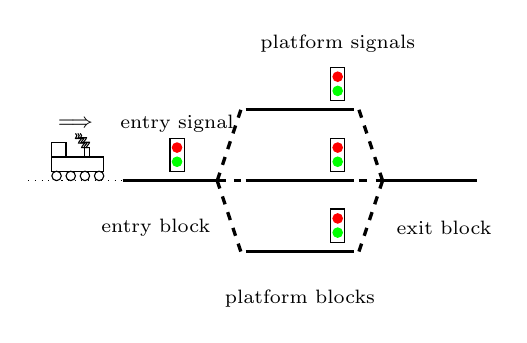
\begin{tikzpicture}[scale=0.6]
  \scriptsize
  % approaching block.
  \draw[very thick] (0,0) -- (1.5,0);
  \draw (0.7, -1) node{entry block};

  % in-switch
  \draw[very thick] (1.5,0) -- (2,0);
  \draw[very thick, dashed] (2,0) -- (2.5,1.5);
  \draw[very thick, dashed] (2,0) -- (2.5,-1.5);
  \draw[very thick, dashed] (2,0) -- (2.5,0);
%  \draw[red] (2, -1.5) node{in-switch};
  
  % platform blocks
  \draw[very thick] (2.6,0) -- (4.9,0);
%  \draw[very thick, dotted] (2.6,0.5) -- (4.9,0.5);
%  \draw[very thick, dotted] (2.6,-0.5) -- (4.9,-0.5);
  \draw[very thick] (2.6,1.5) -- (4.9,1.5);
  \draw[very thick] (2.6,-1.5) -- (4.9,-1.5);
  \draw (3.75, -2.5) node{platform blocks};

  % out-switch
  \draw[very thick] (5.5,0) -- (6,0);
  \draw[very thick, dashed] (5,1.5) -- (5.5,0);
  \draw[very thick, dashed] (5,0) -- (5.5,0);
  \draw[ very thick, dashed] (5,-1.5) -- (5.5,0);
%  \draw[red] (5.5, -1.5) node{out-switch};

  % exiting block.
  \draw[very thick] (6.0,0) -- (7.5,0);
  \draw (6.8, -1) node{exit block};

  % entry signal
%  \draw[very thick] (1.45,0) -- (1.45, 1);
  \draw (1, 0.2) rectangle +(0.3,0.7);
  \filldraw[red] (1.15, 0.7) circle (0.1);
  \filldraw[green] (1.15, 0.4) circle (0.1);
  \draw (1.15, 1.2) node{entry signal};

  % platform signals
%  \draw[very thick] (6.05,0) -- (6.05, 1);
  \draw (4.4, 0.2) rectangle +(0.3,0.7);
  \filldraw[red] (4.55, 0.7) circle (0.1);
  \filldraw[green] (4.55, 0.4) circle (0.1);
  \draw (4.55, 2.9) node{platform signals};

  \draw (4.4, 1.7) rectangle +(0.3,0.7);
  \filldraw[red] (4.55, 2.2) circle (0.1);
  \filldraw[green] (4.55, 1.9) circle (0.1);

  \draw (4.4, -1.3) rectangle +(0.3,0.7);
  \filldraw[red] (4.55, -0.8) circle (0.1);
  \filldraw[green] (4.55, -1.1) circle (0.1);

  % The train
  \draw[dotted] (-2,0) -- (0, 0);
  \draw(-1.5,0.2) rectangle +(1.1, 0.3);
  \draw(-1.5,0.5) rectangle +(0.3, 0.3);
  \draw(-0.8,0.5) rectangle +(0.1, 0.2);
  \draw[decorate, decoration={snake, amplitude = 1pt, segment length = 2pt}] (-0.8,0.7) --  (-1,1);
  \draw[decorate, decoration={snake, amplitude = 1pt, segment length = 2pt}] (-0.75,0.7) --  (-0.95,1);
  \draw[decorate, decoration={snake, amplitude = 1pt, segment length = 2pt}] (-0.7,0.7) --  (-0.9,1);
  \draw (-1.4, 0.1) circle (0.1);
  \draw (-1.1, 0.1) circle (0.1);
  \draw (-0.8, 0.1) circle (0.1);
  \draw (-0.5, 0.1) circle (0.1);
  \draw (-1, 1.2) node{$\Longrightarrow$};
\end{tikzpicture}

\ifx\PREAMBLE\UnDef
\end{document}
\else
\fi

  \caption{A signal control system}
  \label{fig:sgnctrl}
\end{wrapfigure}

The network at the station contains an \emph{entry block}, several
\emph{platform blocks} and an \emph{exiting block}, as seen in
Figure~\ref{fig:sgnctrl}.  Trains arrive on the network at the entry
block, then can move into one of the platform blocks before moving to
the exiting block and leaving the network.
% \begin{requirements}
%   \asm{asm:topology}{There is one entry block, many platform blocks and
%     one exiting block, connected together as shown in
%     Figure~\ref{fig:sgnctrl}.}
%   \asm{asm:movement}{Trains travel in one direction from the entry block
%     to the exiting block via a platform block}
% \end{requirements}
In order to control the trains at the station, signals are positioned
at the end of the entry block and each platform block.  The
train drivers are assumed to obey the signals.  The signals are
supposed to change from green to red automatically when a train passes by.
% \begin{requirements}
%   \asm{asm:entry-signal}{There is a light signal at the end of
%     the entry block}\ReqSpacing
%   \asm{asm:platform-signal}{There is a light signal at the end of each
%     platform block}\ReqSpacing
%   \asm{asm:obey-signal}{Trains obey the light signals} \ReqSpacing
%   \asm{asm:signal-to-red}{Signals change from green to red
%     automatically when a train passes by}
% \end{requirements}

The most important properties of the system are that (1) there should be
no collision between trains (\ref{saf:no-collision}), and (2) each train in the network eventually
leaves~(\ref{live:train-leave}).
\begin{requirements}
  \saf{saf:no-collision}{There is at most one train on each block}\ReqSpacing
  \req{live:train-leave}{Each train in the network eventually leaves}
\end{requirements}

\paragraph{Refinement strategy} In the initial model, we abstractly
model the trains in the network, focusing on~\ref{live:train-leave}.
In the first refinement, we introduce the topology of the network.  We
strengthen the model of the system, focusing on~\ref{saf:no-collision}
in the second refinement.  In the third refinement, we introduce the
signals and derive a specification for the controller that manages
these signals.
% As one can see, the liveness requirement, i.e.,
% \ref{live:train-leave}, is taken early in the development and acts as
% a guideline for designing the system.

\subsection{Initial Model}
\label{sec:initial-model}
\newBset[TRAIN]{TRN}
\newBvrb[trains]{trns}
\newBpar[train]{t}
\newBevt{arrive}
\newBevt{depart}
\newBinv[invTrainType]{inv0\_1}

In this initial model, we use a carrier set \TRAIN to denote the set of
trains and a variable \trains to denote the set of trains currently
within the network.  Initially \trains is assigned the empty set.  At
this abstract level, we have two events to model a train arriving at
the station and a train leaving the station as below.
\begin{Bcode}
  % $
  % \variables{\trains}
  % $
  % \Bhspace
  % $
  % \invariants{\invTrainType: & \trains \subseteq \TRAIN}
  % $
  % \Bvspace
  % $
  % \initialisation{\trains \bcmeq \emptyset}
  % $
  % \Bvspace
  $
  \ubeventinline{\arrive}
  {\train}
  {\train \in \TRAIN}
  {}
  {}
  {\trains \bcmeq \trains \bunion \{\train\}}
  $
  \Bhspace
  $
  \ubeventinline{\depart}{\train}{\train \in \TRAIN}{}{}{\trains \bcmeq
    \trains \setminus \{\train\}}
  $
\end{Bcode}

The requirement \ref{live:train-leave} can be specified as a progress
property \Binv{prg0\_1}: $ \train \in \trains \leadsto t \notin
\trains$.  According to \eqref{eq:trans-prop}, \Binv{prg0\_1} is
equivalent to \Binv{prg0\_2}: $\tr \train \in \trains$.  In order to
implement this transient property, we rely on
Theorem~\ref{thm:transient} and add scheduling information for event
\depart as follows.
\begin{Bcode}
  $
  \ubeventinline{\depart}{\train}{\train \in \TRAIN}{\train \in \trains}{}{\trains \bcmeq \trains \setminus \{\train\}}
  $
\end{Bcode}
Here, we design our \depart event to implement the transient property
\Binv{prg0\_2} such that conditions \eqref{eq:SCH} and \eqref{eq:OP}
are trivial.  For condition \eqref{eq:NEG}, it is easy to prove that
\depart establishes the fact $\train \notin \trains$ in one
step.

Since event \arrive will not affect our reasoning about progress
properties (it is always unscheduled), we are going to omit the
refinement of \arrive in the subsequent presentation.

\subsection{First Refinement}
\label{sec:first-refinement}

\newBset[BLOCK]{BLK}
\newBcst{Entry}
\newBcst[PLATFORM]{PLF}
\newBcst{Exit}
\newBaxm[axmBlockType]{axm1\_1}
\newBvrb[location]{loc}
\newBinv[invLocationType]{inv1\_1}
\newBevt{moveout}
\newBevt{movein}

In this refinement, we first introduce the topology of the network
in terms of blocks.  We introduce a carrier set \BLOCK and three
constants \Entry, \PLATFORM, \Exit denoting the entry block, platform
blocks and exit block, respectively.
% \begin{Bcode}
% $
% \axioms[false]{
%   \axmBlockType: & \partition(\BLOCK, \{Entry\}, \PLATFORM, \{Exit\})
% }
% $
% \end{Bcode}
A new variable \location is introduced denoting the location of trains
in the network, constrained by invariant \invLocationType: $\location
\in \trains \tfun \BLOCK$.
% We refine event \arrive to state that the train to arrive at the entry
% block.
% \begin{Bcode}
%   $
%   \ubevent{\arrive}{\train}{\train \notin \trains}{}{}{
%     \ldots \\
%     \location(\train) \bcmeq \Entry
%   }
%   $
% \end{Bcode}

For event \depart, we strengthen the guard to state that a train can
only leave from the exit block.  Subsequently, in order to make sure
that the schedule is stronger than the guard~(condition
\eqref{eq:fis}), we need to strengthen the coarse-schedule
accordingly (see Figure~\ref{fig:1st-ref}).
In order to prove the refinement of \depart, we apply
Theorem~\ref{thm:ref-rep-crs} (coarse-schedule replacing).  In
particular we need to prove the following conditions:
\begin{gather}
  \train \in \trains ~\leadsto~ \train \in \trains
  \land \location.\train = \Exit \label{eq:33}
  \tag{\Binv{prg1\_1}} \\
  \train \in \trains \land \location.\train =
    \Exit ~\un~ \spneg (\train \in \trains) \label{eq:34}
  \tag{\Binv{un1\_2}}
\end{gather}

\begin{figure}[!hbtp]
  \centering
  \begin{Bcode}[\scriptsize]
    $ \ubevent{\depart}{\train}{ \train \in \trains \land
      \location.\train = \Exit } { \train \in \trains \land
      \location.\train = \Exit} {} {\trains \bcmeq \trains \setminus
      \{\train\} \\ \location \bcmeq \{\train\} \domsub \location} $
    \Bhspace[0.1em]
    $
  \ubevent{\moveout}{\train}
  {\train \in \trains \land \location.\train \in \PLATFORM}
  {\train \in \trains \land \location.\train \in \PLATFORM}
  {}
  {\location.\train \bcmeq \Exit}
  $
  \Bhspace[0.1em]
  $
  \ubevent{\movein}{\train}
  {\train \in \trains \land \location.\train = \Entry}
  {\train \in \trains \land \location.\train = \Entry}
  {}
  {\location \bcmsuch \qexists{p}{p \in \PLATFORM}{\location'
    = \location \ovl \{\train \mapsto p\}}}
  $
  \end{Bcode}
  \vspace{-4ex}
  \caption{Events of the first refinement}
  \label{fig:1st-ref}
\end{figure}

From now on, we focus on reasoning about progress properties, e.g.,
\ref{eq:33}, omitting the reasoning about unless properties, e.g.,
\ref{eq:34}.  The readers should be convinced that using
Theorem~\ref{thm:unless}, these unless properties are valid for our
model.  We first apply \eqref{eq:37} to obtain $\train \in \trains
\land \location.\train \neq \Exit ~\leadsto~ \train \in \trains \land
\location.\train = \Exit$ and then apply the transitivity
property~\eqref{eq:transitivity} of the leads-to operator to establish
two progress properties \ref{eq:24} and \ref{eq:25} as follows.
\begin{gather}
  \label{eq:24}
  \train \in \trains \land \location.\train
  \neq \Exit ~\leadsto~ \train \in
  \trains \land \location.\train \in \PLATFORM
  \tag{\Binv{prg1\_3}}\\
  \label{eq:25}
  \train \in \trains \land \location.\train
  \in \PLATFORM ~\leadsto~ \train \in
  \trains \land \location.\train = \Exit
  \tag{\Binv{prg1\_4}}
\end{gather}
Consider \ref{eq:25}, we first apply the ensure-rule
(Theorem~\ref{thm:ensure-rule}) to establish two properties (after
simplification) as follows:
\begin{gather}
  \label{eq:27}
  \train \in \trains \land \location.\train \in \PLATFORM ~\un~
  \train \in \trains \land \location.\train = \Exit
  \tag{\Binv{un1\_5}}\\
  \label{eq:28}
  \tr \train \in \trains \land \location.\train \in
    \PLATFORM
  \tag{\Binv{prg1\_6}}
\end{gather}

We apply Theorem~\ref{thm:transient} to implement \ref{eq:28} by the
new event \moveout which has a weakly-fair scheduling (see
Figure~\ref{fig:1st-ref}).
% \begin{Bcode}[\footnotesize]
%   $
%   \ubevent{\moveout}{\train}
%   {\train \in \trains \land \location.\train \in \PLATFORM}
%   {\train \in \trains \land \location.\train \in \PLATFORM}
%   {}
%   {\location.\train \bcmeq \Exit}
%   $
% \end{Bcode}
The proof that \moveout implements \ref{eq:28} is straightforward and
therefore is omitted.

Similarly, for \ref{eq:24}, we apply the ensure-rule and implementing
the resulting transient property, i.e., $\tr \train \in \trains \land
\location.\train = \Entry$, by event \movein in Figure~\ref{fig:1st-ref}.
%  The first condition first is equivalent to
% \begin{Bcode}
%     $ \train \in \trains \land
%     \location(\train) \neq \Exit \land
%     \location(\train) \notin \PLATFORM ~\leadsto~ \train \in
%   \trains \land \location(\train) \in \PLATFORM $
% \end{Bcode}

% \begin{Bcode}
%     $ \train \in \trains \land
%     \location(\train) = \Entry ~\leadsto~ \train \in
%   \trains \land \location(\train) \in \PLATFORM $
% \end{Bcode}
% applies the ensure rule
% \begin{Bcode}
%   $\train \in \trains \land
%   \location(\train) = \Entry ~\un~ \train \in
%   \trains \land \location(train) \in \PLATFORM $
%   \\
%   $\tr \train \in \trains \land \location(\train) = \Entry \land \neg (\train \in
%   \trains \land \location(\train) \in \PLATFORM)$
% \end{Bcode}
% The transient property can be implemented by the following event
% \begin{Bcode}[\footnotesize]
%   $
%   \ubevent{\movein}{\train}
%   {\train \in \trains \land \location.\train = \Entry}
%   {\train \in \trains \land \location.\train = \Entry}
%   {}
%   {\location \bcmsuch \qexists{p}{p \in \PLATFORM}{\location'
%     = \location \ovl \{\train \mapsto p\}}}
%   $
% \end{Bcode}

% Currently, our model includes the requirements about the topology
% of the network and the possible movement of trains within the network,
% i.e., \ref{asm:topology} and \ref{asm:movement}.

\subsection{Second Refinement}
\label{sec:second-refinement}
In this refinement, we incorporate the safety requirement stating that
there are no collisions between trains within the network,
i.e. \ref{saf:no-collision}.  This is captured by invariant
\Binv{inv2\_1} about \location: $\qforall{\train_1,\train_2}{\train_1, \train_2 \in \trains \land \location.\train_1 =
  \location.\train_2}{\train_1 = \train_2}$.
% Safety: No collision is model by injectivity property of \location.
% \begin{Bcode}
%   $
%   \invariants{
%     \location \in \trains \pinj \BLOCK
%   }
%   $
% \end{Bcode}
% Event \arrive is refined straightforward
% \begin{Bcode}
%   $
%   \ubevent{\arrive}{\train}{\train \notin \trains \\ \Entry \notin \ran(\location) }{}{}{
%     \trains \bcmeq \trains \bunion \{\train\} \\
%     \location(\train) \bcmeq \Entry
%   }
%   $
% \end{Bcode}

The guard of event \moveout needs to be strengthened to maintain
\Binv{inv2\_1}.  As a result, we need to modify the schedule
information to ensure the \emph{feasibility} condition~\eqref{eq:fis}
for \unitb events stating that the schedules are stronger than the
guard.  In particular, we add (through strengthening) a fine-schedule to
\moveout (see Figure~\ref{fig:2nd-ref}).
\begin{figure}[!htbp]
  \centering
  \begin{Bcode}[\scriptsize]
    $ \ubevent{\moveout}{\train}{ \train \in \trains \land
      \location.\train \in \PLATFORM \land \\
      \Exit \notin \ran.\location
    }{\train \in \trains \land \location.\train \in \PLATFORM} {\Exit
      \notin \ran.\location} {\location.\train \bcmeq \Exit} $
    \Bhspace
  $
  \ubevent{\movein}{\train}
  {\train \in \trains \land \location.\train = \Entry \land
    \qexists{p}{p \in \PLATFORM}{p \notin \ran.\location}
  }
  {\train \in \trains \land \location.\train = \Entry  \land     \qexists{p}{p \in \PLATFORM}{p \notin \ran.\location}}
  {}
  {\location \bcmsuch \qexists{p}{p \in \PLATFORM \setminus 
    \ran.\location}{\location'
    = \location \ovl \{\train \mapsto p\}}}
  $
  \end{Bcode}
  \vspace{-4ex}
  \caption{Events of the second refinement}
  \label{fig:2nd-ref}
\end{figure}
The scheduling information for \moveout states that for any train
$\train$, if $\train$ stays in a platform for infinitely long and the
exit block becomes free infinitely often, then $\train$ can move out of the
platform.

%\marginpar{Simon: Rephrase this paragraph if possible}
We want to highlight the fact that \moveout has both coarse- and
fine-schedules.  In particular, using only either weak- or
strong-fairness would be unsatisfactory.
Weak-fairness requires for the exit block to be remain free continuously in order for
trains to move out.  This assumption is not met by the current system.
Strong-fairness allows a train to leave if the train is present on the
platform intermittently.  This assumption is more flexible than we
need since it allows behaviours where a train hops on and off
the platform infinitely often. The price of that flexibility is to entangle 
properties of the exit block with properties of trains: indeed, we would
need not only to prove that the train will be on its platform and that 
the exit block will become free but that both happen simultaneously
infinitely often.

%\todo{Son: (to SImon) We need to make this point clearer. What I want
%  to focus here is that coarse-/fine-schedules are suitable
%  specification rather than weak-/strong-fairness.}
We choose to relinquish this flexibility and are therefore capable of structuring
our proof better: on one hand, the train stays on its platform as
long as necessary; independently, the exit block becomes free
infinitely many times. 

In order to prove the refinement of \moveout, we apply
Theorem~\ref{thm:strengthen-fns} (fine-schedule strengthening), which
requires to prove the following progress property (remember that when
an event has no fine schedules, it is assumed to be $\one$).
\begin{equation}
  \label{eq:31}
  \one \leadsto \Exit \notin \ran.\location
  \tag{\Binv{prg2\_3}}
\end{equation}
Property
\ref{eq:31} is equivalent to transient property \Binv{prg2\_4}: $\tr
\Exit \in \ran.\location$.  We satisfy \Binv{prg2\_4} by applying the
transient rule (Theorem~\ref{thm:transient}) using event \depart where
the value for the parameter $\train$ is given by
$\location^{-1}.\Exit$, i.e., the train at the exit block.  The
proofs of conditions~\eqref{eq:SCH}, \eqref{eq:OP}, and \eqref{eq:NEG} are
straight-forward.

Finally we strengthen the guard of \movein and subsequently strengthen
its coarse-schedule (see Figure~\ref{fig:2nd-ref}).  We apply
Theorem~\ref{thm:ref-rep-crs} (coarse-schedule replacing) \movein.
The detailed proof is omitted here.

\subsection{Third Refinement}
\label{sec:third-refinement}

\newBset{COLOR}
\newBcst[GREEN]{GR}
\newBcst[RED]{RD}
\newBvrb[signal]{sgn}
\newBevt[ctrlplf]{ctrl\_platform}
\newBpar[platform]{p}

In this refinement, we introduce the signals associated with different
blocks within the network.  Variable \signal is introduced to denote
the value of the signals associated with different blocks.  We focus
on the controlling of the platform signals here.  In particular,
invariants \Binv{inv3\_2} and \Binv{inv3\_3} state that if a platform signal is
green (\GREEN) then the exit block is free and the other platform
signals are red (\RED).
  \begin{Bcode}[\footnotesize]
    $ \invariants[false]{ \Binv{inv3\_1}: & \signal \in \{\Entry\}
      \bunion \PLATFORM \tfun
      \COLOR \\
      \Binv{inv3\_2}: & \qforall{p}{p \in \PLATFORM \land \signal.p =
        \GREEN}{\Exit \notin \ran.\location} \\
      \Binv{inv3\_3}: & \qforall{p,q}{p, q \in \PLATFORM \land
        \signal.p = \signal.q = \GREEN}{p = q} } $
  \end{Bcode}

\begin{figure}[!htbp]
  \centering
  \begin{Bcode}[\scriptsize]
    $
    \ubevent{\moveout}{\train}{
      \train \in \trains \land
      \location.\train \in \PLATFORM \land \\
      \signal.(\location.\train) = \GREEN
    }{\train \in \trains \land \location.train \in \PLATFORM \land \\
    \signal.(\location.\train) = \GREEN}{}{\location.\train \bcmeq
    \Exit \\
    \signal.(\location.\train) \bcmeq \RED
  }
  $
  \Bhspace
  $
  \ubevent{\ctrlplf}{\platform}{
    \platform \in \PLATFORM \land
    \platform \in \ran.\location \land
    \Exit \notin \ran.\location \land \\
    \qforall{q}{q \in \PLATFORM}{\signal.q = \RED}
  }
  {
    \platform \in \PLATFORM \land
    \platform \in \ran.\location \land
    \signal.\platform = \RED
  }
  {
    \Exit \notin \ran(\location) \land
    \qforall{q}{q \in \PLATFORM \land q \neq \platform}{\signal.q = \RED}
  }
  {\signal.\platform \bcmeq \GREEN}
  $
\end{Bcode}
\vspace{-4ex}
\caption{Events of the third refinement}
\label{fig:3rd-ref}
\end{figure}
We refine the \moveout event using the platform signal as shown in Figure~\ref{fig:3rd-ref}.
The refinement of \moveout is justified by applying
Theorem~\ref{thm:ref-rep-crs} (coarse-schedule replacing) and
Theorem~\ref{thm:remove-fns} (fine-schedule removing).  In particular,
replacing the coarse-schedule requires the following transient
property
% \begin{equation}
%   \label{eq:99}
%   \train \in \trains \land \location.\train \in \PLATFORM
%   \wide\leadsto \train \in \trains \land \location.\train \in
%   \PLATFORM \land \signal.(\location.\train) = \GREEN~,
%   \tag{\Binv{prg3\_4}}
% \end{equation}
% which can be implemented by
\begin{equation}
  \label{eq:35}
  \tr \train \in \trains \land \location.\train \in
  \PLATFORM \land \signal.(\location.\train) = \RED~.
  \tag{\Binv{prg3\_5}}
\end{equation}

In order to satisfy \ref{eq:35}, we introduce a new event
\ctrlplf for the controller to change a platform signal to green according to
Theorem~\ref{thm:transient} (see Figure~\ref{fig:3rd-ref}).
% \begin{Bcode}[\footnotesize]
%   $
%   \ubevent{\ctrlplf}{\platform}{
%     \platform \in \PLATFORM \land
%     \platform \in \ran.\location \land
%     \Exit \notin \ran.\location \land
%     \qforall{q}{q \in \PLATFORM}{\signal.q = \RED}
%   }
%   {
%     \platform \in \PLATFORM \land
%     \platform \in \ran.\location \land
%     \signal.\platform = \RED
%   }
%   {
%     \Exit \notin \ran(\location) \land
%     \qforall{q}{q \in \PLATFORM \land q \neq \platform}{\signal.q = \RED}
%   }
%   {\signal.\platform \bcmeq \GREEN}
%   $
% \end{Bcode}
This event \ctrlplf is a specification for the system to control the
platform signals preserving both safety and liveness properties of the
system.  In particular, the scheduling information states that if (1)
a platform is occupied and the platform signal is \RED infinitely long
and (2) the exit block is unoccupied and the other platform signals
are all \RED infinitely often, then the system should eventually set
this platform signal to \GREEN.
The refinement of event \movein and how the entry signal is controlled
is similar and omitted.

%%% Local Variables: 
%%% mode: latex
%%% TeX-master: "progress"
%%% End: 


%% !TEX root = progress-llncs.tex
% \section{Related Work}
% \label{sec:related-work}

%%%%% Event-B
% Our \unitb method is inspired by \eventB and \unity.  We borrow the
% idea of refining specifications (transition systems) from \eventB and
% extending it to address liveness properties.  
\unitb and \eventB differ mainly in the scheduling
assumptions.  In \eventB, event executions are assumed to
satisfy the \emph{minimal progress} condition: as long
as there are events that are enabled, one will be chosen non-
deterministically. %
%\todo{Son: (to Simon) Check the definition of minimal progress}%
Given this assumption, certain liveness properties can be proved
for \eventB models such as \emph{progress} and
\emph{persistence}~\cite{hoang11:_reason_liven_proper_event_b}.
However, this work does not discuss how the refinement notion can be
adapted to preserve liveness properties.  Moreover, the
minimum progress assumption is often either too weak to prove
liveness properties or, when it's not, make the proofs needlessly 
complicated.

%   Often, one needs to have stronger assumptions
% such as weak- or strong-fairness.
%
%%%%% UNITY
% Our temporal logic reasoning is inspired by the \unity logic.
% Operators such as $\tr$ and $\un$ are defined within
% \unity~\cite{DBLP:books/daglib/0067338}.  What we have done is to give
% definition to these operators using computation calculus and to prove
% several properties related to these operators.  The main difference
% between \unitb and \unity is in the method.  In \unitb, we gradually
% refine the model (the transition system) in a property-preserving
% manner.  In \unity, a specification is essentially a property and a
% program is a transition system.  In \unitb, we unify
% the notions of specifications and programs, allowing them to be
% evolved together during refinement.
%
%%%%% The notion of fairness
% A key important feature of \unitb is the introduction of the notion of
% coarse-schedule and fine-schedule.  They are more general than the
% standard weak- and strong-fairness assumptions that has been used in
% many methods including \unity and
% TLA+~\cite{DBLP_books_aw_Lamport2002}.  As illustrated by our example
% in Section~\ref{sec:second-refinement} and
% Section~\ref{sec:third-refinement}, in some cases, event scheduling
% information can be captured quite naturally using coarse- and
% fair-schedules, while this would not be straightforward to be captured
% by weak- or strong-fairness assumptions.
%
%%%%% TLA+
TLA+\cite{DBLP_books_aw_Lamport2002} is another formal method based on
refinement and which supports liveness properties.  The
execution of a TLA+ model is also captured as a formula with safety
and liveness sub-formulae.  However, refinement of the liveness part
in TLA+ involves calculating explicitly the fairness assumptions of the
abstract and concrete models.  This is not practical in our
opinion for developing realistic systems in general.  The
lack of practical rules for refining the liveness part in TLA+ might be
rooted in the view of the author of TLA+ concerning the
\emph{unimportance of liveness}~\cite[Chapter
8]{DBLP_books_aw_Lamport2002}.  In our opinion, liveness
properties are as important as safety properties to design
correct systems.

%%% Local Variables: 
%%% mode: latex
%%% TeX-master: "progress"
%%% End: 


\section{Conclusion}
\label{sec:conclusion}

We presented in this paper \unitb, a formal method inspired by \eventB
and \unity.  Our method allows systems to be developed gradually via
refinement and support reasoning about both safety and liveness
properties.  An important feature of \unitb is the notion of coarse-
and fine-schedules for events.  Standard weak- and strong-fairness
assumptions can be expressed using these event schedules.  We
proposed refinement rules to manipulate the coarse-
and fine-schedules such that liveness properties are
preserved.  We illustrated \unitb by developing a signal control
system.

A key observation in \unitb is the role of event scheduling regarding
liveness properties being similar to the role of guards regarding safety
properties.  Guards prevents events to occur in some unsafe state such
that safety properties cannot be violated.  Schedules ensure event
occurrences such that liveness properties can be satisfied.  Another
key aspect of \unitb is the role of progress properties during
refinement.  Often, to ensure the validity of a refinement, one needs
to prove some progress properties which (eventually) can be
``implemented'' (satisfied) by some scheduled events.

\paragraph{Related work}
% !TEX root = progress-llncs.tex
% \section{Related Work}
% \label{sec:related-work}

%%%%% Event-B
% Our \unitb method is inspired by \eventB and \unity.  We borrow the
% idea of refining specifications (transition systems) from \eventB and
% extending it to address liveness properties.  
\unitb and \eventB differ mainly in the scheduling
assumptions.  In \eventB, event executions are assumed to
satisfy the \emph{minimal progress} condition: as long
as there are events that are enabled, one will be chosen non-
deterministically. %
%\todo{Son: (to Simon) Check the definition of minimal progress}%
Given this assumption, certain liveness properties can be proved
for \eventB models such as \emph{progress} and
\emph{persistence}~\cite{hoang11:_reason_liven_proper_event_b}.
However, this work does not discuss how the refinement notion can be
adapted to preserve liveness properties.  Moreover, the
minimum progress assumption is often either too weak to prove
liveness properties or, when it's not, make the proofs needlessly 
complicated.

%   Often, one needs to have stronger assumptions
% such as weak- or strong-fairness.
%
%%%%% UNITY
% Our temporal logic reasoning is inspired by the \unity logic.
% Operators such as $\tr$ and $\un$ are defined within
% \unity~\cite{DBLP:books/daglib/0067338}.  What we have done is to give
% definition to these operators using computation calculus and to prove
% several properties related to these operators.  The main difference
% between \unitb and \unity is in the method.  In \unitb, we gradually
% refine the model (the transition system) in a property-preserving
% manner.  In \unity, a specification is essentially a property and a
% program is a transition system.  In \unitb, we unify
% the notions of specifications and programs, allowing them to be
% evolved together during refinement.
%
%%%%% The notion of fairness
% A key important feature of \unitb is the introduction of the notion of
% coarse-schedule and fine-schedule.  They are more general than the
% standard weak- and strong-fairness assumptions that has been used in
% many methods including \unity and
% TLA+~\cite{DBLP_books_aw_Lamport2002}.  As illustrated by our example
% in Section~\ref{sec:second-refinement} and
% Section~\ref{sec:third-refinement}, in some cases, event scheduling
% information can be captured quite naturally using coarse- and
% fair-schedules, while this would not be straightforward to be captured
% by weak- or strong-fairness assumptions.
%
%%%%% TLA+
TLA+\cite{DBLP_books_aw_Lamport2002} is another formal method based on
refinement and which supports liveness properties.  The
execution of a TLA+ model is also captured as a formula with safety
and liveness sub-formulae.  However, refinement of the liveness part
in TLA+ involves calculating explicitly the fairness assumptions of the
abstract and concrete models.  This is not practical in our
opinion for developing realistic systems in general.  The
lack of practical rules for refining the liveness part in TLA+ might be
rooted in the view of the author of TLA+ concerning the
\emph{unimportance of liveness}~\cite[Chapter
8]{DBLP_books_aw_Lamport2002}.  In our opinion, liveness
properties are as important as safety properties to design
correct systems.

%%% Local Variables: 
%%% mode: latex
%%% TeX-master: "progress"
%%% End: 


\paragraph{Future work}

%%%%% Data refinement
Currently, we only consider superposition refinement in \unitb where
variables are retained during refinement.  More generally, variables
can be removed and replaced by other variables during refinement (data
refinement). We are working on extending \unitb to provide rules for data
refinement.

%%%%% Decomposition/Composition 
Another important technique for coping with the difficulties in
developing complex systems is composition/decomposition and is already
a part of methods such as \eventB and \unity.  We intend to investigate
on how this technique can be added to \unitb, in particular, the role
of event scheduling during composition/decomposition.

%%%%% Tool support
Given the close relationship between \unitb and \eventB, we are
looking at extending the supporting Rodin
platform~\cite{abrial10:_rodin} of \eventB to accomodate \unitb.  We
expect to generate the corresponding proof obligations according to
different refinement rules such that it can be verified using the
existing provers of Rodin.


%%% Local Variables: 
%%% mode: latex
%%% TeX-master: "progress"
%%% End: 


\bibliographystyle{plain}
\bibliography{progress}

%\newpage
%\listoftodos
\end{document}


%%% Local Variables: 
%%% mode: latex
%%% TeX-master: "progress"
%%% End: 
